% Báo cáo thực tập: nghiên cứu bài toán dự đoán cảm xúc Hi-EF.
% Dựa trên template khóa luận VNU-UET (https://github.com/DoHaiSon/Graduate_Thesis), giữ nguyên định dạng trang,
% phông chữ và kiểu đề mục; bỏ apacite/harvard, dùng natbib + BibTeX (references.bib).
\documentclass[a4paper,12pt,oneside]{book}
\usepackage{times}
\usepackage{appendix}
\usepackage[shortlabels]{enumitem}
\usepackage{booktabs}
\usepackage{hhline}
\usepackage{colortbl}
\usepackage{afterpage}
\usepackage{mathtools}
\usepackage{setspace}
\usepackage[utf8]{vietnam}
\usepackage{amstext,amsmath,latexsym,amsbsy,amssymb,amsthm,amsfonts,multicol,nccmath}
\usepackage[left=3cm,right=2cm,top=2.5cm,bottom=3cm,footskip=40pt]{geometry}
\usepackage{pdflscape}
\usepackage{tikz}
\usetikzlibrary{calc}
\usepackage{array}
\newcolumntype{C}[1]{>{\centering\let\newline\\\arraybackslash\hspace{0pt}}m{#1}}
\usepackage{tabularx}
\usepackage{xcolor}
\setcounter{secnumdepth}{4}
\usepackage[square,comma,numbers,sort&compress]{natbib}
\setlength{\parindent}{1cm}
\usepackage{indentfirst}
\usepackage{exscale,eucal}
\usepackage{fancyhdr}
\usepackage{fncychap}
\usepackage[chapter]{algorithm}
\usepackage{multirow}
\usepackage{graphicx}
\usepackage{algpseudocode}
\usepackage{longtable}
\usepackage{etoolbox}
\usepackage{titlesec}
\usepackage[labelsep=period]{caption}
\usepackage{subfigure}
\DeclareCaptionFormat{myformat}{\fontsize{13}{15}\selectfont#1#2#3}
\captionsetup{format=myformat}
\usepackage{titletoc}
\titlelabel{\thetitle.\,\,}
\titleformat{\chapter}[display]
  {\fontsize{14}{16}\selectfont\bfseries\centering}
  {\MakeUppercase{\chaptertitlename}\ \thechapter}{0pt}{\fontsize{14}{16}\selectfont\MakeUppercase}
\titlespacing{\chapter}{0pt}{0pt}{40pt}
\titleformat*{\section}{\fontsize{14}{14}\selectfont\bfseries}
\titleformat*{\subsection}{\fontsize{14}{14}\selectfont\bfseries\slshape}
\titleformat*{\subsubsection}{\fontsize{14}{14}\slshape}
\titleformat*{\paragraph}{\large\bfseries}
\titleformat*{\subparagraph}{\large\bfseries}
\graphicspath{{figures/}}
\titlespacing\section{0pt}{6pt plus 4pt minus 2pt}{1pt plus 2pt minus 2pt}
\titlespacing\subsection{0pt}{6pt plus 4pt minus 2pt}{1pt plus 2pt minus 2pt}
\titlespacing\subsubsection{0pt}{6pt plus 4pt minus 2pt}{0pt plus 2pt minus 2pt}
\usepackage[subfigure]{tocloft}
\cftsetpnumwidth{20pt}
\titlecontents{chapter}
  [0pt]
  {}
  {\fontsize{13.5}{14}\selectfont\MakeUppercase{\chaptername}\ \thecontentslabel.\,\,}
  {}
  {\cftdotfill{\cftdotsep}\contentspage}
\renewcommand{\cftsecaftersnum}{.}
\renewcommand{\cftsubsecaftersnum}{.}
\newtheorem{definition}{\bf Định nghĩa}[chapter]
\renewcommand{\cftfigfont}{Hình~}
\renewcommand{\cfttabfont}{Bảng~ }
\floatname{algorithm}{Thuật toán}
\renewcommand{\algorithmicrequire}{\textbf{Đầu vào:}}
\makeatletter
\renewcommand\@biblabel[1]{[#1]}
\makeatother
\flushbottom
\renewcommand*{\bibfont}{\fontsize{13}{16}\selectfont}
\usepackage[hidelinks,unicode]{hyperref}

% ký hiệu dùng chung
\newcommand{\model}{RoleNet}
% chỗ dành cho kết quả của các notebook đang chạy (G46a, G47, G48); xóa khi đã điền số liệu
\newcommand{\choketqua}[1]{{\color{red}\itshape [Chờ kết quả: #1]}}

\begin{document}
% Thứ tự theo Quy định trình bày KLTN (Trường ĐH Công nghệ): bìa, phụ bìa tiếng Việt, tóm tắt, lời cam đoan, mục lục, ký hiệu và chữ viết tắt, nội dung, phụ lục, tài liệu tham khảo.
% Chữ 13pt, giãn dòng 1,3, cách đoạn 6pt, thụt đầu dòng 1 cm; lề 2,5/3/3/2 cm (geometry ở trên).
\fontsize{13}{15}\selectfont
\pagestyle{empty}
\begin{titlepage}
    \centering
\begin{tikzpicture}[overlay,remember picture]
\centering
\draw[line width = 3pt] ($(current page.north west) + (1.215in,-0.7in)$) rectangle ($(current page.south east) + (-0.7in,0.7in)$);
\draw (0,-24.5) node[above]{\fontsize{12}{12}\selectfont{\textbf{HÀ NỘI -- [NĂM]}}};
\end{tikzpicture}
\vspace{-1cm}
\begin{center}
\MakeUppercase{\textbf{\fontsize{12}{12}\selectfont{Đại học quốc gia hà nội}}}

\noindent{\textbf {\MakeUppercase{\fontsize{12}{12}\selectfont {trường đại học công nghệ}}}}\\
\vspace{1.5cm}
\begin{figure}[!htb]
	\centering
	
\includegraphics[width=0.2\linewidth]{figures/UET_logo.jpg}
\end{figure}
\vspace{1.5cm}

{\textbf {\fontsize{14}{14}\selectfont{[HỌ VÀ TÊN SINH VIÊN]}}}\\
\vspace{2cm}
{\textbf {\MakeUppercase{\fontsize{17}{17}\selectfont{Nghiên cứu bài toán dự đoán cảm xúc}}}}\\[3pt]
{\textbf {\MakeUppercase{\fontsize{17}{17}\selectfont{trong hội thoại đa phương thức Hi-EF}}}}\\[3pt]
\vspace{3cm}
\MakeUppercase{\textbf{\fontsize{14}{14}\selectfont{Báo cáo thực tập}}}\\[3pt]
{\fontsize{14}{14}\textbf{\selectfont{Ngành: [TÊN NGÀNH]}}}
\end{center}
\end{titlepage}

% Phụ lục 02 của quy định: trang phụ bìa tiếng Việt
\begin{titlepage}
\centering
{\fontsize{12}{14}\selectfont\textbf{ĐẠI HỌC QUỐC GIA HÀ NỘI}\\
\textbf{TRƯỜNG ĐẠI HỌC CÔNG NGHỆ}\par}
\vspace{2.2cm}
{\fontsize{14}{16}\selectfont\textbf{[Họ và tên sinh viên]}\par}
\vspace{2.2cm}
{\fontsize{18}{24}\selectfont\textbf{NGHIÊN CỨU BÀI TOÁN DỰ ĐOÁN CẢM XÚC\\TRONG HỘI THOẠI ĐA PHƯƠNG THỨC HI-EF}\par}
\vspace{2.6cm}
{\fontsize{14}{16}\selectfont\textbf{BÁO CÁO THỰC TẬP}\\[4pt]
\textbf{Ngành: [Tên ngành đào tạo]}\par}
\vspace{2.4cm}
\raggedright\leftskip=1.2cm
{\fontsize{14}{16}\selectfont\textbf{Cán bộ hướng dẫn: [Học hàm, học vị, họ tên]}\par}
{\fontsize{11}{13}\selectfont\itshape (ký tên)\par}
\vspace{1.6cm}
{\fontsize{14}{16}\selectfont\textbf{Cán bộ đồng hướng dẫn: [nếu có]}\par}
{\fontsize{11}{13}\selectfont\itshape (ký tên)\par}
\vspace{1.0cm}
{\fontsize{14}{16}\selectfont\textbf{Đơn vị thực tập: [Tên đơn vị]}\par}
\vfill
\centering
{\fontsize{12}{14}\selectfont\textbf{HÀ NỘI -- 20[..]}\par}
\vspace*{0.3cm}
\noindent\begin{tikzpicture}[overlay,remember picture]
\draw[line width = 3pt] ($(current page.north west) + (1.215in,-0.7in)$) rectangle ($(current page.south east) + (-0.7in,0.7in)$);
\end{tikzpicture}
\end{titlepage}

\pagestyle{plain}
\pagenumbering{roman}
\setstretch{1.3}
\setlength{\parindent}{1cm}
\setlength{\parskip}{6pt}
\clearpage
\phantomsection
\addcontentsline{toc}{chapter}{Tóm tắt}
\chapter*{\fontsize{13}{15}\selectfont{Tóm tắt}}
\fontsize{12}{12}\selectfont{
\noindent\textbf{Tóm tắt:}
Dự đoán cảm xúc trong hội thoại là bài toán ước lượng một người sẽ cảm thấy thế nào ở lượt nói tiếp theo, trước khi lượt nói đó diễn ra. Bộ dữ liệu Hi-EF đặt bài toán này trên video phim truyền hình: từ ba đoạn hội thoại liên tiếp, mô hình phải dự đoán cảm xúc của người sẽ nói ở đoạn thứ tư, trong khi danh tính người đó không được cho trước. Báo cáo trình bày quá trình nghiên cứu bài toán, từ phân tích dữ liệu, tái lập mô hình gốc, đến đề xuất mô hình \model{}. \model{} chọn một người nghe làm đại diện cho người sẽ phản hồi mà không dùng thông tin tương lai, biểu diễn mỗi người trong mỗi lượt bằng một token bằng chứng và dùng một bộ mã hóa tập hợp nhỏ (0,71 triệu tham số) để dự đoán. Trên tập kiểm tra được khóa và chỉ đánh giá một lần theo kế hoạch đăng ký trước, \model{} tăng UAR từ 21,40 lên 25,24 và WAR từ 32,52 lên 36,43 so với mô hình gốc được huấn luyện lại; chỉ số chính đã đăng ký trước (UAR sau hiệu chỉnh logit) tăng tương tự nhưng không có ý nghĩa thống kê. Các phân tích có kiểm soát trên dữ liệu phát triển cho thấy khuôn mặt của người nghe và ngữ cảnh của các lượt trước là hai nguồn thông tin quan trọng nhất, mỗi nguồn đóng góp khoảng hai điểm UAR; người nghe được chọn tự động cho kết quả tương đương người phản hồi thật hay một người không nói được chọn ngẫu nhiên, và nhãn vai trò không tạo khác biệt đo được; và lợi thế của mô hình tập trung ở các trường hợp người phản hồi lặp lại cảm xúc của người nói hoặc giữ cảm xúc của chính mình. Báo cáo cũng trình bày các hướng đã thử nhưng không thành công và rút ra rằng giới hạn hiện tại nằm ở việc nhận diện trạng thái cảm xúc của những người tham gia.

\vspace{0.5cm}
\noindent\textbf{\textit{Từ khóa:}} \textit{dự đoán cảm xúc, hội thoại đa phương thức, Hi-EF, người nghe.}
}

\fontsize{13}{15}\selectfont
\clearpage
\phantomsection
\addcontentsline{toc}{chapter}{Lời cam đoan}
\chapter*{Lời cam đoan}

Tôi xin cam đoan báo cáo thực tập \textbf{Nghiên cứu bài toán dự đoán cảm xúc trong hội thoại đa phương thức Hi-EF} là kết quả làm việc của tôi trong thời gian thực tập tại [TÊN ĐƠN VỊ], dưới sự hướng dẫn của [HỌC HÀM, HỌC VỊ, HỌ TÊN].

Các số liệu và kết quả trình bày trong báo cáo được tạo ra từ các thực nghiệm do tôi thực hiện; mã nguồn và nhật ký chạy được lưu lại để có thể kiểm tra. Các phương pháp, bộ dữ liệu và công cụ của tác giả khác đều được trích dẫn đầy đủ. Những kết quả không đạt kỳ vọng cũng được báo cáo trung thực, kèm điều kiện thực nghiệm tương ứng.

Nếu có gì sai trái, tôi xin hoàn toàn chịu trách nhiệm.

\vspace{1cm}
\hspace{7cm}\textit{Hà Nội, ngày ... tháng ... năm [NĂM]}

\hspace{9.4cm}\textbf{Sinh viên}
\vspace{2.5cm}

\hspace{8.8cm}\textbf{[HỌ VÀ TÊN SINH VIÊN]}

\clearpage
\phantomsection
\addcontentsline{toc}{chapter}{Lời cảm ơn}
\chapter*{Lời cảm ơn}

\textit{Tôi xin chân thành cảm ơn [HỌC HÀM, HỌC VỊ, HỌ TÊN], người đã hướng dẫn và định hướng cho tôi trong suốt thời gian thực tập. Tôi cũng xin cảm ơn [TÊN ĐƠN VỊ] đã tạo điều kiện về môi trường làm việc và tài nguyên tính toán, cùng các thầy cô [TÊN KHOA] đã trang bị cho tôi những kiến thức nền tảng để thực hiện đề tài này.}

\textit{[Lời cảm ơn bổ sung, nếu có.]}

\vspace{1cm}
\hspace{7cm}\textit{Hà Nội, ngày ... tháng ... năm [NĂM]}

\hspace{9.4cm}\textbf{Sinh viên}
\vspace{2.5cm}

\hspace{8.8cm}\textbf{[HỌ VÀ TÊN SINH VIÊN]}


\fontsize{13}{15}\selectfont
\renewcommand{\contentsname}{\vspace{-70pt}\centerline{\fontsize{14}{16}\selectfont\MakeUppercase{Mục lục}}}
\clearpage
\phantomsection
\addcontentsline{toc}{chapter}{Mục lục}
\tableofcontents
\clearpage
\clearpage
\phantomsection
\addcontentsline{toc}{chapter}{Danh mục ký hiệu và chữ viết tắt}
\chapter*{Danh mục ký hiệu và chữ viết tắt}
{\renewcommand{\arraystretch}{1.4}
{\fontsize{12}{13}\selectfont
\begin{longtable}{|C{0.8cm}|>{\raggedright}p{3.6cm}|p{9.8cm}|}
\hline
\multicolumn{3}{|l|}{\textbf{Danh mục ký hiệu}}\\
\hline\hline
\textbf{STT} & \textbf{Ký hiệu} & ~\hfill\textbf{Giải thích}\hfill~\\
\hline
1&A&Người nói của clip III\\
\hline
2&B&Người phản hồi, tức người nói của clip IV (cần dự đoán cảm xúc)\\
\hline
3&L&Người nghe được chọn làm đại diện cho B (listener proxy)\\
\hline
4&O&Những người còn lại trong cảnh\\
\hline
5&$k$&Chỉ số clip, $k \in \{1,2,3\}$ ứng với clip I, II, III\\
\hline
6&$x_{r,k}$&Token khuôn mặt của vai trò $r$ trong clip $k$\\
\hline
7&$s_k$, $g_k$&Token lời nói và token bối cảnh của clip $k$\\
\hline
8&$q$&Token truy vấn dùng để đọc kết quả dự đoán\\
\hline
9&$\phi(f)$&Vector đặc trưng 146 chiều của một khuôn mặt $f$\\
\hline
10&$p(y_B \mid X)$&Phân phối dự đoán cảm xúc của B khi biết ba clip đầu vào\\
\hline
11&$d$&Số chiều ẩn của mô hình ($d = 128$)\\
\hline
\end{longtable}
}}
{\renewcommand{\arraystretch}{1.2}
{\fontsize{12}{13}\selectfont
\begin{longtable}{|C{0.8cm}|p{1.7cm}|>{\raggedright}p{5.5cm}|p{5.75cm}|}
\hline
\multicolumn{4}{|l|}{\textbf{Danh mục chữ viết tắt}}\\
\hline\hline
\textbf{STT} & \textbf{Viết tắt} & \textbf{Giải thích tiếng Anh} & \textbf{Giải thích tiếng Việt}\\
\hline
1&CI&Confidence Interval&Khoảng tin cậy\\
\hline
2&CLIP&Contrastive Language--Image Pre-training&Mô hình học tương phản ảnh -- văn bản\\
\hline
3&CV&Cross-Validation&Kiểm định chéo\\
\hline
4&ECAPA&Emphasized Channel Attention, Propagation and Aggregation&Mạng nhúng giọng nói ECAPA-TDNN\\
\hline
5&EMAP&Empirical Multimodally-Additive Projection&Phép chiếu cộng tính thực nghiệm đa phương thức\\
\hline
6&ERC&Emotion Recognition in Conversation&Nhận diện cảm xúc trong hội thoại\\
\hline
7&FFN&Feed-Forward Network&Mạng truyền thẳng\\
\hline
8&Hi-EF&Hi-EF benchmark&Bộ dữ liệu dự đoán cảm xúc trong tương tác đa lớp\\
\hline
9&LA&Logit Adjustment&Hiệu chỉnh logit theo tần suất lớp\\
\hline
10&LN&Layer Normalization&Chuẩn hóa theo lớp\\
\hline
11&MCIS&Multilayered-Contextual Interaction Sample&Mẫu tương tác ngữ cảnh đa lớp\\
\hline
12&MELD&Multimodal EmotionLines Dataset&Bộ dữ liệu cảm xúc đa phương thức MELD\\
\hline
13&MHA&Multi-Head Attention&Chú ý đa đầu\\
\hline
14&MLP&Multi-Layer Perceptron&Mạng nơ-ron nhiều lớp\\
\hline
15&NLL&Negative Log-Likelihood&Hàm hợp lý âm\\
\hline
16&OOF&Out-of-Fold&Dự đoán ngoài fold\\
\hline
17&PCA&Principal Component Analysis&Phân tích thành phần chính\\
\hline
18&PMA&Pooling by Multihead Attention&Gộp bằng chú ý đa đầu\\
\hline
19&SAB&Set Attention Block&Khối chú ý trên tập hợp\\
\hline
20&UAR&Unweighted Average Recall&Độ nhạy trung bình không trọng số\\
\hline
21&WAR&Weighted Average Recall&Độ chính xác (độ nhạy trung bình có trọng số)\\
\hline
\end{longtable}
}}

\clearpage
\phantomsection
\addcontentsline{toc}{chapter}{Danh mục hình vẽ}
\renewcommand{\listfigurename}{\vspace{-70pt}\centerline{\fontsize{14}{16}\selectfont{\MakeUppercase{Danh mục hình vẽ}}}}
\listoffigures
\clearpage
\phantomsection
\addcontentsline{toc}{chapter}{Danh mục bảng biểu}
\renewcommand{\listtablename}{\vspace{-70pt}\centerline{\fontsize{14}{16}\selectfont{\MakeUppercase{Danh mục bảng biểu}}}}
\listoftables
\clearpage

% số trang Ả-rập liên tục từ Mở đầu đến hết phần sau cùng, ở giữa cuối trang
\pagenumbering{arabic}
\pagestyle{plain}
\fontsize{13}{15}\selectfont

\clearpage
\phantomsection
\addcontentsline{toc}{chapter}{Mở đầu}
\chapter*{Mở đầu}

\noindent{\Large\textbf{Lý do chọn đề tài}}

Cảm xúc chi phối cách con người phản ứng với nhau trong hội thoại. Phần lớn các nghiên cứu về cảm xúc trong hội thoại giải quyết bài toán \emph{nhận diện}: gán nhãn cảm xúc cho một câu nói hoặc một đoạn video đã quan sát được. Trong nhiều ứng dụng như trợ lý ảo, robot xã hội hay hệ thống hỗ trợ tư vấn, điều cần biết lại là một người \emph{sắp} cảm thấy thế nào, để hệ thống có thể điều chỉnh cách phản hồi trước khi phản ứng đó xảy ra. Đây là bài toán \emph{dự đoán cảm xúc} (emotion forecasting): thông tin về lượt nói cần dự đoán hoàn toàn chưa có, mô hình chỉ được nhìn vào những gì đã diễn ra trước đó.

Bộ dữ liệu Hi-EF \cite{wang2026hief} được công bố gần đây đưa bài toán này vào bối cảnh video đa phương thức. Mỗi mẫu gồm bốn đoạn video liên tiếp trích từ phim truyền hình; ba đoạn đầu là đầu vào, và nhiệm vụ là dự đoán cảm xúc của người nói ở đoạn thứ tư. Bài toán có hai điểm khó đặc biệt. Thứ nhất, đoạn thứ tư không bao giờ được quan sát. Thứ hai, danh tính của người sẽ nói ở đoạn thứ tư, tức người phản hồi, không được cho biết. Mô hình gốc của Hi-EF xử lý mỗi đoạn như một khối thống nhất rồi gộp theo thời gian, nên bằng chứng bị chi phối bởi người đang nói, trong khi người sắp phản hồi thường đã xuất hiện trên màn hình với vai trò người nghe.

Vì bộ dữ liệu còn mới, chưa có nhiều phân tích về việc thông tin nào thật sự giúp dự đoán, cũng như về độ tin cậy của các con số được báo cáo. Đề tài này chọn Hi-EF làm đối tượng nghiên cứu nhằm hiểu rõ bài toán, xây dựng một mô hình phù hợp với cấu trúc của hội thoại nhiều người, và đánh giá nó theo một quy trình chặt chẽ.

\vspace{0.3cm}
\noindent{\Large\textbf{Mục tiêu nghiên cứu}}

\renewcommand{\labelitemi}{$-$}
\begin{itemize}
	\item Phân tích bộ dữ liệu Hi-EF: ai có mặt trong mỗi mẫu, người phản hồi xuất hiện ở đâu, và những quy luật nào liên hệ cảm xúc của người phản hồi với ngữ cảnh.
	\item Tái lập mô hình tốt nhất của bài báo gốc trên một cách chia dữ liệu không rò rỉ giữa các tập.
	\item Đề xuất một mô hình dự đoán tổ chức bằng chứng xoay quanh những người tham gia hội thoại, đặc biệt là người nghe.
	\item Xác định bằng các thực nghiệm có kiểm soát xem phần cải thiện đến từ đâu, và giới hạn hiện tại của bài toán nằm ở đâu.
\end{itemize}

\vspace{0.3cm}
\noindent{\Large\textbf{Phương pháp nghiên cứu}}

Đề tài kết hợp khảo sát tài liệu, phân tích dữ liệu và thực nghiệm có kiểm soát. Mọi quyết định thiết kế được đưa ra trên dữ liệu phát triển bằng kiểm định chéo theo tập phim (episode), để không có đoạn video nào xuất hiện đồng thời trong dữ liệu huấn luyện và đánh giá. Tập kiểm tra được khóa, và kết quả chính trên tập này được đọc đúng một lần theo một kế hoạch đã cam kết trước khi chạy (preregistration), gồm mô hình, số seed, chỉ số và thứ tự các phép so sánh. Mỗi thực nghiệm được viết thành một notebook có quy tắc đọc kết quả cố định từ trước, chạy trên Kaggle, và được chạy thử với dữ liệu giả trước khi chạy thật. Các khác biệt được đánh giá bằng bootstrap theo seed và theo tập phim.

\vspace{0.3cm}
\noindent{\Large\textbf{Nội dung nghiên cứu}}

\begin{itemize}
	\item Tìm hiểu các bài toán nhận diện và dự đoán cảm xúc trong hội thoại, bộ dữ liệu Hi-EF và các bộ trích xuất đặc trưng khuôn mặt, giọng nói, văn bản.
	\item Trích xuất lại đặc trưng mức khuôn mặt và giọng nói, phân tích thống kê về người tham gia trong Hi-EF.
	\item Xây dựng mô hình \model{} và so sánh với mô hình gốc trên Hi-EF và trên MELD.
	\item Thực hiện các phân tích loại bỏ thành phần (ablation), so sánh người nghe đại diện với người phản hồi thật, kiểm tra nguồn gốc của phần cải thiện và phân tích lỗi.
	\item Thử nghiệm và đánh giá các hướng cải tiến khác, ghi nhận cả những hướng không thành công.
\end{itemize}

\vspace{0.3cm}
\noindent{\Large\textbf{Đóng góp của đề tài}}

\begin{itemize}
	\item Một quy tắc chọn người nghe làm đại diện cho người phản hồi, không dùng thông tin tương lai, nhãn người nói hay chú thích danh tính.
	\item Mô hình \model{} biểu diễn ba đoạn ngữ cảnh thành một tập token theo người và theo lượt, đọc bằng một bộ mã hóa tập hợp nhỏ; mô hình có khoảng 40 lần ít tham số hơn mô hình gốc.
	\item Kết quả trên tập kiểm tra được khóa: UAR tăng 3,84 điểm so với mô hình gốc huấn luyện lại, thắng ở bảy trên tám tập phim kiểm tra.
	\item Một loạt phân tích có kiểm soát mô tả phần cải thiện: vai trò của người nghe và của ngữ cảnh, so sánh với người phản hồi thật, so sánh với mô hình gốc dùng cùng đặc trưng, và phân biệt hai hiện tượng lặp lại cảm xúc người nói (mirroring) và giữ cảm xúc của chính mình (persistence).
\end{itemize}

\vspace{0.3cm}
\noindent{\Large\textbf{Bố cục của báo cáo}}

\begin{itemize}
	\item \textbf{Chương 1} trình bày tổng quan về nhận diện và dự đoán cảm xúc trong hội thoại, bộ dữ liệu Hi-EF, các bộ trích xuất đặc trưng, mô hình trên tập hợp và các phương pháp đánh giá.
	\item \textbf{Chương 2} phân tích dữ liệu: cách chia tập, phân bố nhãn, những người có mặt trong mỗi mẫu và các quy luật cảm xúc.
	\item \textbf{Chương 3} mô tả mô hình \model{}.
	\item \textbf{Chương 4} trình bày thiết lập thực nghiệm, kết quả chính và các phân tích.
	\item \textbf{Chương 5} tổng hợp các hướng đã thử nhưng không thành công và bài học rút ra.
	\item \textbf{Kết luận} tóm tắt kết quả, các hạn chế và hướng phát triển.
\end{itemize}

\newpage
\clearpage
\phantomsection
\setcounter{chapter}{0}
\chapter[TỔNG QUAN VÀ CƠ SỞ LÝ THUYẾT]{Tổng quan và cơ sở lý thuyết}

Chương này giới thiệu các khái niệm và công cụ mà báo cáo sử dụng: bài toán nhận diện và dự đoán cảm xúc trong hội thoại, bộ dữ liệu Hi-EF cùng mô hình gốc của nó, các bộ trích xuất đặc trưng được dùng để mô tả khuôn mặt, giọng nói và lời thoại, kiến trúc Transformer áp dụng cho dữ liệu dạng tập hợp, và các phương pháp đánh giá.

\section{Nhận diện cảm xúc trong hội thoại}

Bài toán nhận diện cảm xúc trong hội thoại (Emotion Recognition in Conversation, ERC) gán cho mỗi câu nói trong một cuộc hội thoại một nhãn cảm xúc. Các nhãn thường theo bộ cảm xúc cơ bản gồm tức giận (\emph{angry}), ghê sợ (\emph{disgust}), sợ hãi (\emph{fear}), vui (\emph{happy}), buồn (\emph{sad}), ngạc nhiên (\emph{surprise}) cùng nhãn trung tính (\emph{neutral}). Điểm khác biệt với nhận diện cảm xúc trên từng câu độc lập là ngữ cảnh: cảm xúc của một câu phụ thuộc vào những gì đã được nói trước đó và vào việc ai đang nói.

Các mô hình ERC tiêu biểu xây dựng bộ nhớ hoặc đồ thị theo người nói. ICON \cite{hazarika2018icon} lưu trạng thái riêng cho từng người và mô hình hóa ảnh hưởng qua lại giữa họ. DialogueRNN \cite{majumder2019dialoguernn} cập nhật một trạng thái cho mỗi bên tham gia sau mỗi câu nói của họ. DialogueGCN \cite{ghosal2019dialoguegcn} biểu diễn hội thoại bằng đồ thị có cạnh theo quan hệ giữa người nói. Với dữ liệu đa phương thức, MulT \cite{tsai2019mult} dùng chú ý chéo giữa các luồng văn bản, âm thanh và hình ảnh. Bộ dữ liệu MELD \cite{poria2019meld}, xây dựng từ phim \emph{Friends}, là chuẩn đánh giá phổ biến cho ERC đa phương thức nhiều người; MELD cung cấp tên người nói cho từng câu.

Điểm chung của các phương pháp này là giả định danh tính người nói đã biết. Giả định đó hợp lý khi nhận diện cảm xúc của những câu đã xảy ra, nhưng không còn đúng trong bài toán dự đoán của Hi-EF, nơi danh tính người sẽ nói tiếp theo không được cho trước.

\section{Dự đoán cảm xúc}

\subsection{Khái niệm}

Trong tâm lý học, dự đoán cảm xúc (affective forecasting) nghiên cứu cách con người ước lượng cảm xúc tương lai của chính mình \cite{wilson2003affective}. Trong học máy, bài toán được phát biểu như sau: cho chuỗi các lượt hội thoại đã quan sát, ước lượng cảm xúc của một lượt chưa xảy ra. \citet{wang2020sentiment} nghiên cứu dự đoán cảm xúc tích cực -- tiêu cực của lượt kế tiếp trong hội thoại văn bản. Khác với nhận diện, mô hình dự đoán không có bất kỳ tín hiệu nào từ chính lượt cần dự đoán: không có khuôn mặt, giọng nói hay lời thoại của lượt đó. Mọi thông tin phải được suy ra từ những gì đã diễn ra.

\subsection{Hai quy luật của cảm xúc trong hội thoại}

Hai hiện tượng được nghiên cứu nhiều trong tâm lý học gợi ý những nguồn thông tin hữu ích cho việc dự đoán.

\textbf{Lây lan cảm xúc} (emotional contagion) \cite{hatfield1994contagion}: người tham gia hội thoại có xu hướng tiếp nhận cảm xúc của người đối diện, thông qua việc bắt chước nét mặt, giọng nói và tư thế. Trong dữ liệu hội thoại, hiện tượng này thể hiện qua việc người phản hồi có cùng cảm xúc với người vừa nói. Báo cáo gọi các trường hợp này là \emph{mirroring}.

\textbf{Quán tính cảm xúc} (emotional inertia) \cite{kuppens2010inertia}: trạng thái cảm xúc của một người có xu hướng duy trì theo thời gian, tức cảm xúc ở thời điểm sau phụ thuộc vào cảm xúc ở thời điểm trước của chính người đó. Báo cáo gọi các trường hợp người phản hồi giữ nguyên cảm xúc của chính mình ở lượt trước là \emph{persistence}.

Cả hai quy luật đều đi qua người phản hồi: lây lan cảm xúc có thể quan sát qua phản ứng của người đó khi đang nghe, còn quán tính cảm xúc có thể quan sát qua những biểu hiện trước đó của chính người đó. Đây là cơ sở để xây dựng mô hình xoay quanh người phản hồi ở Chương 3.

\section{Bộ dữ liệu Hi-EF và mô hình gốc}

Hi-EF \cite{wang2026hief} là bộ dữ liệu dự đoán cảm xúc trong tương tác, được xây dựng từ video phim truyền hình. Mỗi mẫu được gọi là một MCIS (multilayered-contextual interaction sample) gồm bốn đoạn video liên tiếp, mỗi đoạn ứng với một câu phụ đề:

\begin{itemize}
	\item clip I và clip II: ngữ cảnh trước đó;
	\item clip III: lượt nói của người nói A;
	\item clip IV: lượt nói của một người khác, người phản hồi B.
\end{itemize}

Nhiệm vụ là dự đoán cảm xúc của B trong clip IV, thuộc một trong bảy lớp kể trên, chỉ dựa vào video, âm thanh và phụ đề của ba clip đầu. Danh tính của B không được cho trước. Bài báo gốc trình bày bài toán dưới dạng tương tác hai người A -- B; Chương 2 sẽ cho thấy trên thực tế phần lớn các mẫu có nhiều hơn hai người.

Mô hình tốt nhất trong bài báo gốc, báo cáo này gọi là \emph{mô hình gốc} hay \emph{baseline}, xử lý từng clip bằng hai bộ mã hóa thời gian kiểu Transformer trên chuỗi 16 khung hình (đặc trưng CLIP của toàn khung hình và của khuôn mặt), kết hợp với đặc trưng văn bản và âm thanh bằng chú ý chéo, rồi gộp ba clip bằng một mạng LSTM ba lớp và một Transformer. Mô hình có khoảng 27,7 triệu tham số. Đơn vị xử lý của mô hình là cả khung hình và cả clip, nên thông tin về từng người trong cảnh bị trộn lẫn.

\section{Các bộ trích xuất đặc trưng}

Báo cáo sử dụng các mô hình đã được huấn luyện sẵn và giữ cố định để trích xuất đặc trưng. Phần này tóm tắt vai trò của từng mô hình.

\textbf{ArcFace} \cite{deng2019arcface} là mô hình nhận dạng khuôn mặt, ánh xạ mỗi khuôn mặt thành một vector 512 chiều sao cho các khuôn mặt của cùng một người có độ tương đồng cosine cao. Mô hình được huấn luyện với hàm mất mát có biên góc cộng (additive angular margin), giúp tách biệt các danh tính trên mặt cầu đơn vị. Báo cáo dùng ArcFace để gom các khuôn mặt trong một mẫu thành các danh tính, không gắn tên cho bất kỳ ai.

\textbf{HSEmotion} \cite{savchenko2022hsemotion} là mô hình nhận diện biểu cảm khuôn mặt dựa trên EfficientNet, cho ra xác suất của tám biểu cảm, hai giá trị valence (mức độ tích cực) và arousal (mức độ kích thích), cùng một vector nhúng 1280 chiều. Đây là nguồn mô tả nét mặt chính của mô hình đề xuất.

\textbf{CLIP} \cite{radford2021clip} học một không gian chung cho ảnh và văn bản bằng học tương phản trên các cặp ảnh -- chú thích. Bộ đặc trưng đi kèm Hi-EF dùng CLIP để mã hóa khung hình, khuôn mặt và phụ đề.

\textbf{AudioCLIP} \cite{guzhov2022audioclip} mở rộng CLIP sang âm thanh. Đặc trưng âm thanh trong bộ dữ liệu là vector 527 chiều ứng với các lớp sự kiện âm thanh của AudioSet, nghĩa là mô tả loại âm thanh chứ không chuyên về ngữ điệu hay cảm xúc trong giọng nói.

\textbf{ECAPA-TDNN} \cite{desplanques2020ecapa} là mạng nhúng giọng nói dùng cho nhận dạng người nói. Báo cáo dùng nó để so sánh giọng giữa các clip, từ đó suy ra ai có khả năng đang nói mà không cần biết tên người nói.

\section{Transformer và mô hình trên tập hợp}

\subsection{Cơ chế tự chú ý}

Transformer \cite{vaswani2017attention} xử lý một dãy token $H \in \mathbb{R}^{n \times d}$ bằng cơ chế tự chú ý. Với các phép chiếu $Q = HW_Q$, $K = HW_K$, $V = HW_V$, đầu ra của một đầu chú ý là
\begin{equation}
	\mathrm{Attn}(Q, K, V) = \operatorname{softmax}\!\left(\frac{QK^\top}{\sqrt{d_k}}\right) V .
\end{equation}
Chú ý đa đầu (MHA) chạy song song nhiều đầu như vậy rồi ghép kết quả. Mỗi lớp Transformer gồm một khối MHA và một mạng truyền thẳng (FFN), mỗi khối có kết nối tắt và chuẩn hóa theo lớp (LN). Chi phí của một lớp là $O(n^2 d + n d^2)$.

\subsection{Mô hình trên tập hợp}

Khi đầu vào là một tập hợp không có thứ tự, mô hình nên cho kết quả không đổi khi hoán vị các phần tử. Deep Sets \cite{zaheer2017deep} chứng minh rằng mọi hàm bất biến hoán vị có thể biểu diễn dưới dạng $\rho\big(\sum_i \psi(x_i)\big)$. Set Transformer \cite{lee2019set} dùng chú ý để mô hình hóa tương tác giữa các phần tử. Khối chú ý trên tập hợp (Set Attention Block, SAB) chính là một lớp Transformer \emph{không} có mã hóa vị trí, nên đầu ra hoán vị theo đúng cách hoán vị của đầu vào (đồng biến hoán vị). Để thu được một vector đại diện cho cả tập, Set Transformer dùng phép gộp bằng chú ý đa đầu (PMA): một số vector "hạt giống" học được truy vấn vào tập. Chương 3 dùng cách nhìn này: bằng chứng của một mẫu được biểu diễn thành một tập token, và một token truy vấn đóng vai trò hạt giống để đọc ra dự đoán.

\section{Phương pháp đánh giá}

\subsection{Các chỉ số}

Gọi $y_i$ là nhãn thật, $\hat y_i$ là nhãn dự đoán và $\mathcal{C}$ là tập bảy lớp. Độ nhạy của lớp $c$ là tỉ lệ mẫu thuộc lớp $c$ được dự đoán đúng. Hai chỉ số chính theo bài báo gốc là
\begin{equation}
	\mathrm{UAR} = \frac{1}{|\mathcal{C}|}\sum_{c \in \mathcal{C}} \frac{|\{i: y_i = c, \hat y_i = c\}|}{|\{i: y_i = c\}|}, \qquad
	\mathrm{WAR} = \frac{|\{i: \hat y_i = y_i\}|}{N}.
\end{equation}
UAR (độ nhạy trung bình không trọng số) đối xử với mọi lớp như nhau nên phạt mô hình chỉ dự đoán các lớp đông; WAR chính là độ chính xác. Vì các lớp trong Hi-EF mất cân bằng, UAR là chỉ số chính của báo cáo. Với một mô hình đoán ngẫu nhiên đều, UAR bằng $1/7 \approx 14{,}29$.

\textbf{Hiệu chỉnh logit} (logit adjustment, LA) \cite{menon2021logit} bù cho sự mất cân bằng lớp ở bước suy luận: thay vì chọn lớp có xác suất lớn nhất, ta chọn
\begin{equation}
	\hat y = \arg\max_{c} \big(\log p(c \mid x) - \tau \log \pi_c\big),
\end{equation}
với $\pi_c$ là tần suất lớp $c$ trên tập huấn luyện và $\tau = 1$. Phép hiệu chỉnh này nâng các lớp hiếm lên.

\textbf{Hàm hợp lý âm} (NLL) đo chất lượng của toàn bộ phân phối dự đoán chứ không chỉ nhãn được chọn. Vì các mô hình mạng nơ-ron thường quá tự tin, xác suất được hiệu chỉnh bằng temperature scaling \cite{guo2017calibration}, tức chia logit cho một hằng số $T$ học trên dữ liệu giữ lại, trước khi tính NLL. NLL được dùng cho các so sánh cấu trúc có hiệu ứng nhỏ.

\subsection{Kiểm định chéo theo tập phim}

Các clip trong cùng một tập phim có cùng nhân vật, bối cảnh và ánh sáng; các MCIS liên tiếp còn có thể dùng chung clip. Nếu chia ngẫu nhiên theo mẫu, mô hình có thể "nhớ" nhân vật và cho kết quả lạc quan. Vì vậy mọi phép chia trong báo cáo đều theo tập phim: một tập phim chỉ thuộc về đúng một phía. Kiểm định chéo 5 fold được thực hiện trên các tập phim của dữ liệu phát triển; trong mỗi fold, năm tập phim của phần huấn luyện được giữ riêng để dừng sớm. Mọi bước có học từ dữ liệu, kể cả phép PCA trên đặc trưng khuôn mặt, chỉ được thực hiện trên phần huấn luyện của fold.

\subsection{Đánh giá độ bất định bằng bootstrap}

Kết quả của mạng nơ-ron thay đổi theo seed khởi tạo, và tập đánh giá chỉ có vài chục tập phim. Báo cáo dùng \emph{bootstrap hai mức} để đánh giá khác biệt giữa hai mô hình: trong mỗi lần lặp, lấy mẫu có hoàn lại các seed của từng mô hình rồi lấy trung bình xác suất dự đoán (tạo một ensemble), và lấy mẫu có hoàn lại các tập phim để tính chỉ số. Khoảng giữa phân vị 2,5\% và 97,5\% sau 2.000 lần lặp là khoảng tin cậy 95\%. Một khác biệt được coi là có ý nghĩa khi cận dưới của khoảng này lớn hơn 0.

\subsection{Đăng ký trước kế hoạch đánh giá}

Khi cùng một tập kiểm tra được dùng nhiều lần để chọn mô hình, con số cuối cùng sẽ lạc quan hơn thực tế. Để tránh điều đó, báo cáo áp dụng \emph{đăng ký trước} (preregistration): trước khi mở tập kiểm tra, các mô hình, số seed, chỉ số chính và thứ tự các phép so sánh được ghi lại và cam kết; tập kiểm tra sau đó được đọc đúng một lần. Ngoài ra, mỗi thực nghiệm trên dữ liệu phát triển đều có một quy tắc đọc kết quả được cố định trước khi chạy, để kết luận không bị điều chỉnh sau khi đã thấy số liệu.

\newpage
\clearpage
\phantomsection
\chapter[DỮ LIỆU VÀ PHÂN TÍCH DỮ LIỆU]{Dữ liệu và phân tích dữ liệu}

Trước khi thiết kế mô hình, cần hiểu rõ dữ liệu: các tập được chia thế nào, nhãn phân bố ra sao, và quan trọng nhất là trong mỗi mẫu có những ai, người phản hồi xuất hiện ở đâu. Các phân tích trong chương này được thực hiện trên dữ liệu phát triển; clip IV chỉ được dùng để phân tích, không bao giờ làm đầu vào cho mô hình dự đoán.

\section{Bộ dữ liệu Hi-EF và cách chia tập}

Bộ chú thích công bố của Hi-EF gồm 2.830 MCIS lấy từ 53 tập phim. Mỗi clip dài khoảng hai giây và ứng với một câu phụ đề. Cách chia tập của bài báo gốc cho phép các MCIS của cùng một tập phim, thậm chí dùng chung clip, nằm ở cả tập huấn luyện lẫn tập kiểm tra. Để tránh rò rỉ, báo cáo chia lại theo tập phim với tỉ lệ 37/8/8 tập phim, tương ứng 1.993/428/409 MCIS cho huấn luyện, kiểm định và kiểm tra. Hai tập huấn luyện và kiểm định được gộp thành \emph{dữ liệu phát triển} gồm 45 tập phim và 2.421 MCIS, dùng cho mọi thực nghiệm kiểm định chéo. Tập kiểm tra gồm 8 tập phim được khóa lại. Do cách chia khác, các con số trong báo cáo không so sánh trực tiếp được với con số trong bài báo gốc; thay vào đó, mô hình gốc được huấn luyện lại trên cùng cách chia (Mục~\ref{sec:thietlap}).

\begin{table}[!htb]
\centering
\caption{Phân bố nhãn cảm xúc của B trong clip IV}
\label{tab:phanbo}
\begin{tabular}{lrrrr}
\toprule
 & \multicolumn{2}{c}{Phát triển (45 tập phim)} & \multicolumn{2}{c}{Kiểm tra (8 tập phim)} \\
\cmidrule(lr){2-3}\cmidrule(lr){4-5}
Cảm xúc & Số mẫu & Tỉ lệ (\%) & Số mẫu & Tỉ lệ (\%) \\
\midrule
angry & 448 & 18,5 & 77 & 18,8 \\
disgust & 220 & 9,1 & 40 & 9,8 \\
fear & 32 & 1,3 & 6 & 1,5 \\
happy & 562 & 23,2 & 100 & 24,4 \\
neutral & 563 & 23,3 & 89 & 21,8 \\
sad & 359 & 14,8 & 60 & 14,7 \\
surprise & 237 & 9,8 & 37 & 9,0 \\
\midrule
Tổng & 2.421 & 100 & 409 & 100 \\
\bottomrule
\end{tabular}
\end{table}

Bảng~\ref{tab:phanbo} cho thấy phân bố nhãn của hai phía khá giống nhau, nhưng mất cân bằng mạnh: \emph{happy} và \emph{neutral} chiếm gần một nửa, trong khi \emph{fear} chỉ có 32 mẫu phát triển và 6 mẫu kiểm tra. Với 6 mẫu, mỗi dự đoán đúng thêm một mẫu \emph{fear} làm UAR trên tập kiểm tra thay đổi 2,38 điểm. Điều này ảnh hưởng trực tiếp đến cách đọc kết quả ở Chương 4.

\section{Ai có mặt trong mỗi mẫu}

Bài báo gốc mô tả bài toán như một tương tác hai người. Để kiểm tra giả định này, các khuôn mặt trong mỗi mẫu được phát hiện ở tốc độ 4 khung hình mỗi giây (tối đa 32 khung hình mỗi clip), nhúng bằng ArcFace và gom cụm thành các danh tính; giọng nói được so sánh bằng ECAPA. Người phản hồi B được xác định, chỉ cho mục đích phân tích, là khuôn mặt chiếm ưu thế trong clip IV, sau đó đối chiếu với các danh tính của clip I--III. Hình~\ref{fig:datastats} tóm tắt kết quả.

\begin{figure}[!htb]
\centering
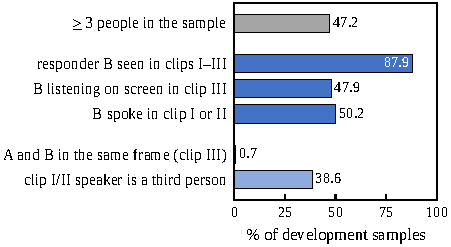
\includegraphics[width=0.75\linewidth]{data_stats.pdf}
\caption{Thống kê người tham gia trong dữ liệu phát triển của Hi-EF (khuôn mặt: 600 mẫu; giọng nói: 592 mẫu; người phản hồi xuất hiện trong clip I--III và đã nói ở clip I/II: 2.421 mẫu; clip IV chỉ dùng để phân tích)}
\label{fig:datastats}
\end{figure}

Có bốn quan sát chính.

\textbf{Hi-EF thực chất là hội thoại nhiều người.} 47\% số mẫu có từ ba người trở lên xuất hiện trong cảnh.

\textbf{Người phản hồi thường đã có mặt từ trước.} B xuất hiện ở clip I--III trong 88\% số mẫu, được thấy đang nghe trong clip III ở 48\% số mẫu, và đã nói ở clip I hoặc II trong 50\% số mẫu. Như vậy, phần lớn thời gian mô hình có thể quan sát trực tiếp người mà nó cần dự đoán.

\textbf{Phim được dựng theo kiểu cắt cảnh luân phiên.} A và B chỉ cùng xuất hiện trong một khung hình của clip III ở 0,7\% số mẫu: máy quay quay người nói, rồi cắt sang người nghe. Hệ quả là một vector tóm tắt mức khung hình hay mức clip sẽ trộn lẫn những người khác nhau.

\textbf{Lượt lời không đủ để xác định B.} Người nói ở clip I/II là một người thứ ba (không phải A, cũng không phải B) trong khoảng 39\% số mẫu, nên quy tắc "người nói trước A chính là B" sai khá thường xuyên.

Một thí nghiệm không cần huấn luyện cho thấy nét mặt của người nghe có thông tin hữu ích. Trên 1.234 mẫu có người nghe nhìn thấy được, chỉ dùng biểu cảm khuôn mặt (HSEmotion) của người nghe để đoán nhãn của B cho UAR cao hơn 3,72 điểm so với dùng biểu cảm của A; trong khi đó, một cờ cho biết người nghe có mặt hay không thì không mang thông tin. Ngoài ra, khoảng một nửa số khung hình có người nghe nằm ở 20\% cuối của clip III, tức rất gần lượt nói cần dự đoán. Chương 4 sẽ kiểm tra liệu mô hình có chỉ dựa vào những khung hình cuối này hay không.

\section{Lặp lại cảm xúc và giữ cảm xúc}

Hai quy luật trình bày ở Chương 1 có thể đo trực tiếp trên nhãn.

\textbf{Mirroring.} Cảm xúc của B trùng với cảm xúc của A trong clip III ở 35,5\% số mẫu phát triển; trên MELD tỉ lệ tương ứng là 34,7\%. Nếu hai nhãn độc lập, tỉ lệ trùng chỉ khoảng 18\%, nên lây lan cảm xúc là một tín hiệu mạnh.

\textbf{Persistence.} Ở 27\% số mẫu phát triển (654 MCIS), B đã nói ở clip I hoặc II và lượt nói đó có nhãn, nên biết được cảm xúc trước đó của chính B. Trong các mẫu này, B giữ nguyên cảm xúc của mình ở clip IV trong 48,9\% trường hợp.

Để có mốc so sánh, Bảng~\ref{tab:copy} liệt kê một số bộ dự đoán chẩn đoán. Hai bộ "sao chép" dùng nhãn thật của ngữ cảnh nên là \emph{oracle}, chỉ dùng để phân tích, không phải là mô hình có thể triển khai. Đường cơ sở dự đoán lớp đông nhất có UAR thấp hơn $1/7$ vì lớp đông nhất khác nhau giữa các fold.

\begin{table}[!htb]
\centering
\caption{Các bộ dự đoán chẩn đoán trên dữ liệu phát triển (kiểm định chéo 5 fold); oracle dùng nhãn thật của ngữ cảnh}
\label{tab:copy}
\begin{tabular}{lcccc}
\toprule
 & \multicolumn{2}{c}{Toàn bộ (2.421)} & \multicolumn{2}{c}{Biết cảm xúc trước của B (654)} \\
\cmidrule(lr){2-3}\cmidrule(lr){4-5}
Bộ dự đoán & UAR & WAR & UAR & WAR \\
\midrule
Lớp đông nhất của fold huấn luyện & 10,82 & 17,60 & 10,55 & 19,57 \\
Sao chép cảm xúc của A (oracle) & 27,12 & 35,52 & 26,18 & 35,93 \\
Sao chép cảm xúc trước của B (oracle) & -- & -- & 39,18 & 48,93 \\
\midrule
Mô hình gốc & 21,27 & 31,68 & 22,74 & 36,39 \\
\model{} & 26,62 & 37,92 & 27,39 & 41,90 \\
\bottomrule
\end{tabular}
\end{table}

Bảng cho thấy hai điều. Thứ nhất, chỉ cần biết đúng cảm xúc trước của B đã đạt 39,18 UAR, cao hơn nhiều so với mọi mô hình; quán tính cảm xúc là nguồn thông tin rất mạnh nếu nhận diện được trạng thái trước đó của B. Thứ hai, \model{}, dù không được thấy nhãn của A, đạt UAR ngang và WAR cao hơn bộ sao chép cảm xúc của A.

\section{Nhãn không chắc chắn}

Bộ chú thích của Hi-EF có một cột mức độ chắc chắn của nhãn với ba mức: chắc chắn, ranh giới và không chắc chắn. Trong các clip có nhãn, số lượng ba mức lần lượt là 3.587, 559 và 637. Với nhãn của clip IV, 25,8\% thuộc hai mức sau; tỉ lệ này đặc biệt cao ở \emph{sad} (41\%), \emph{disgust} (47\%) và \emph{fear} (56\%), cũng là những lớp khó dự đoán nhất. Như vậy một phần sai số của mọi mô hình đến từ sự mơ hồ của chính nhãn.

\section{Bộ dữ liệu MELD}

Để kiểm tra khả năng tổng quát, báo cáo xây dựng các mẫu theo kiểu Hi-EF từ MELD \cite{poria2019meld}: ba lượt nói liên tiếp, tiếp theo là một lượt của người nói khác, cho 5.405/595/1.341 mẫu huấn luyện/kiểm định/kiểm tra. Tên người nói của MELD không được dùng làm đầu vào, để giữ cùng điều kiện với Hi-EF. MELD bị chi phối bởi lớp \emph{neutral}, chiếm 48\% số mẫu kiểm tra.

\newpage
\clearpage
\phantomsection
\chapter[MÔ HÌNH ĐỀ XUẤT ROLENET]{Mô hình đề xuất RoleNet}
\label{chap:method}

Chương này trình bày mô hình \model{}. Ý tưởng chính rút ra từ Chương 2: người sẽ phản hồi thường đã có mặt trên màn hình với vai trò người nghe, và bằng chứng nên được tổ chức theo từng người thay vì theo cả khung hình hay cả clip.

\section{Phát biểu bài toán}

Cho một MCIS với ba clip đầu vào $X = (C_1, C_2, C_3)$, mỗi clip $C_k$ gồm các khung hình video, âm thanh và phụ đề. Mô hình cần đưa ra phân phối xác suất $p(y_B \mid X)$ trên bảy lớp cảm xúc, với $y_B$ là cảm xúc của người phản hồi B trong clip IV. Ba ràng buộc được giữ trong toàn bộ nghiên cứu: clip IV không bao giờ là đầu vào khi suy luận; danh tính của B không được cho; và không giả định chỉ có hai người tham gia.

\begin{figure}[!htb]
\centering
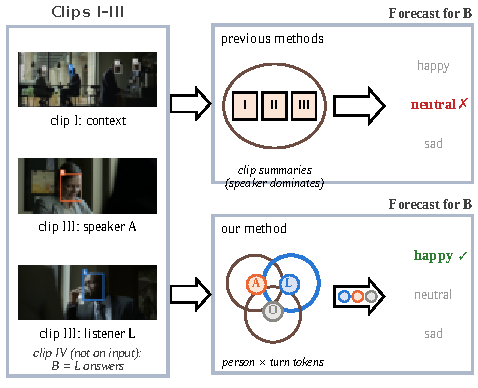
\includegraphics[width=0.62\linewidth]{motivation.pdf}
\caption{Một mẫu kiểm tra của Hi-EF có nhiều người trong cảnh. Bên trái: các vai trò mà \model{} gán mà không dùng thông tin tương lai (người nói A của clip III, người nghe L làm đại diện cho người phản hồi, và những người còn lại O). Bên phải: tóm tắt mỗi clip quanh người nói cho dự đoán \emph{neutral}, còn \model{} xây dựng quanh người nghe dự đoán đúng phản ứng \emph{happy} của B}
\label{fig:motivation}
\end{figure}

\section{Tổng quan kiến trúc}

Hình~\ref{fig:arch} cho thấy cấu trúc của \model{}, gồm bốn bước:

\begin{enumerate}
	\item \textbf{Trích xuất đặc trưng.} Khuôn mặt được phát hiện và mô tả bằng ArcFace và HSEmotion; khung hình và phụ đề bằng CLIP; âm thanh bằng AudioCLIP và ECAPA.
	\item \textbf{Gán vai trò.} Mỗi khuôn mặt được gán một trong ba vai trò: người nói A của clip III, người nghe L làm đại diện cho người phản hồi, và những người còn lại O (Mục~\ref{sec:roles}).
	\item \textbf{Xây dựng tập bằng chứng.} Mỗi cặp (vai trò, clip) được tóm tắt thành một token khuôn mặt; mỗi clip có thêm một token lời nói và một token bối cảnh, tổng cộng 15 token (Mục~\ref{sec:tokens}).
	\item \textbf{Mã hóa tập hợp và dự đoán.} Một bộ mã hóa tập hợp nhỏ đọc cả 15 token cùng lúc, và một token truy vấn gộp chúng thành dự đoán (Mục~\ref{sec:encoder}).
\end{enumerate}

\begin{figure}[!htb]
\centering
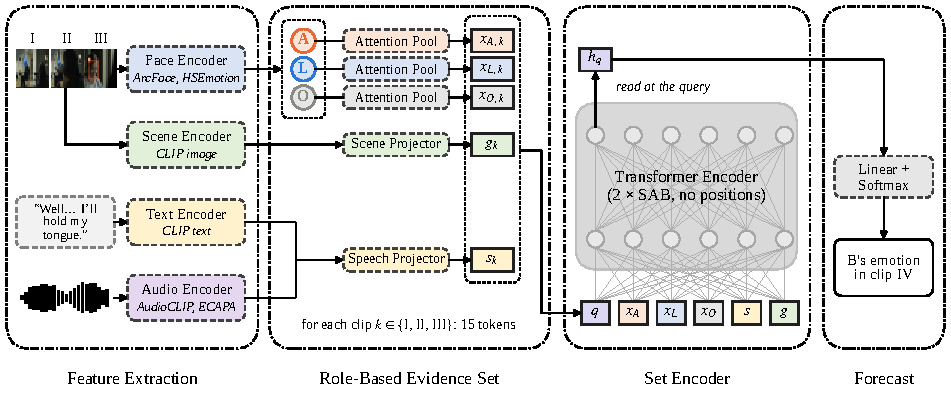
\includegraphics[width=\linewidth]{architecture.pdf}
\caption{Kiến trúc tổng thể của \model{}. Khuôn mặt của clip I--III được gom thành các danh tính; trong clip III, danh tính xuất hiện nhiều nhất là người nói A và danh tính nhiều thứ hai là người nghe L. Mỗi ô vai trò $\times$ clip trở thành một token khuôn mặt, mỗi clip thêm một token lời nói và một token bối cảnh. Token truy vấn gộp tập đã mã hóa thành dự đoán}
\label{fig:arch}
\end{figure}

\section{Gán vai trò}
\label{sec:roles}

Phim truyền hình thường được dựng theo kiểu cảnh -- cảnh phản ứng: máy quay dừng lâu ở người đang nói, rồi cắt sang người đang nghe, thường cũng là người sẽ trả lời. \model{} dựa vào quy ước này để đoán người phản hồi mà không cần thông tin tương lai.

Cụ thể, khuôn mặt được phát hiện trong các khung hình của clip I--III ở tốc độ 4 khung hình mỗi giây (tối đa 32 khung hình mỗi clip) và nhúng bằng ArcFace. Toàn bộ khuôn mặt của một MCIS được gom cụm phân cấp (liên kết trung bình, ngưỡng tương đồng cosine 0,45), sao cho mỗi cụm xấp xỉ một người xuyên suốt ba clip. Trong clip III, cụm có nhiều khung hình nhất được coi là người nói A, cụm nhiều thứ hai là người nghe L; mọi cụm khác là O. Nếu clip III chỉ có một người, mẫu đó không có người nghe. Như vậy mỗi khuôn mặt $f$ nhận một vai trò $r(f) \in \{A, L, O\}$.

Quy tắc này không đọc clip IV, không dùng nhãn người nói hay chú thích danh tính, và không gắn tên cho ai. Các cụm chỉ có ý nghĩa bên trong một mẫu. Trong phân tích ban đầu trên 600 mẫu, người nghe được chọn trùng với người phản hồi thật trong 81,4\% trường hợp; với cách đối chiếu chặt hơn trên toàn bộ dữ liệu phát triển, tỉ lệ này là khoảng 68--73\% trong số các mẫu có người nghe. Mục~\ref{sec:proxy} sẽ cho thấy việc thay L bằng người phản hồi thật không cải thiện dự đoán.

\section{Token bằng chứng}
\label{sec:tokens}

\subsection{Token khuôn mặt}

Mỗi clip của Hi-EF chỉ dài khoảng hai giây, và người nghe thường chỉ xuất hiện trong một đến ba khung hình. Vì vậy \model{} tóm tắt mỗi người trong mỗi clip bằng \emph{một} token, giữ cho tập bằng chứng nhỏ, nhưng vẫn cho phép mô hình tập trung vào khung hình biểu cảm nhất.

Gọi $F_{r,k}$ là tập khung hình (tối đa 24) chứa khuôn mặt có vai trò $r$ trong clip $k$. Mỗi khuôn mặt được mô tả bằng vector $\phi(f) \in \mathbb{R}^{146}$ gồm: 128 thành phần PCA của vector nhúng HSEmotion (PCA chỉ được khớp trên khuôn mặt của dữ liệu huấn luyện trong từng fold), 8 xác suất biểu cảm cùng valence và arousal, hướng đầu, vị trí và kích thước khuôn mặt, độ mở miệng, và thời điểm tương đối của khung hình trong clip. Các khung hình của một ô được gộp bằng chú ý:
\begin{equation}
\begin{split}
u_f &= \mathrm{MLP}(\phi(f)),\\
\alpha_f &= \operatorname{softmax}_{f \in F_{r,k}}\big(w^\top u_f\big),\\
x_{r,k} &= \textstyle\sum_{f} \alpha_f u_f + e^{\text{role}}_r + e^{\text{clip}}_k ,
\end{split}
\label{eq:pool}
\end{equation}
trong đó $e^{\text{role}}_r$ và $e^{\text{clip}}_k$ là các vector nhúng học được của vai trò và của clip. Trọng số $\alpha_f$ cho phép mô hình chọn khung hình mang nhiều thông tin nhất thay vì lấy trung bình đều. Nếu một ô không có khuôn mặt nào, ví dụ người nghe không xuất hiện trong clip I, token được thay bằng một vector giữ chỗ học được $a_{r,k}$. Kết quả là chín token khuôn mặt $x_{r,k} \in \mathbb{R}^d$ với $d = 128$ cho mỗi MCIS.

\subsection{Token lời nói và token bối cảnh}

Những gì được nói và bối cảnh của mỗi lượt bổ sung cho khuôn mặt. Với mỗi clip, \model{} tạo một token lời nói $s_k$ và một token bối cảnh $g_k$:
\begin{align}
s_k &= W_t\,t_k + (W_a\,a_k)\,\delta_k + W_v\,v_k + e^{\text{speech}} + e^{\text{clip}}_k, \label{eq:sk}\\
g_k &= W_s\,[\bar c^{\,\text{frame}}_k;\,\bar c^{\,\text{face}}_k] + e^{\text{scene}} + e^{\text{clip}}_k, \label{eq:gk}
\end{align}
trong đó $t_k$ là vector CLIP của phụ đề, $a_k$ là vector sự kiện âm thanh AudioCLIP nhân với cờ $\delta_k$ cho biết có âm thanh hay không, và $\bar c$ là trung bình vector CLIP của toàn khung hình và của mọi khuôn mặt. Vector mô tả lượt $v_k$ (9 chiều) gồm độ đồng bộ giữa cử động miệng và năng lượng âm thanh của từng vai trò, độ tương đồng giọng nói ECAPA so với clip III, và số danh tính. Vector này giúp mô hình biết ai có khả năng đang nói ở clip I và II mà không cần gọi tên ai.

Cùng nhau, các token khuôn mặt, lời nói và bối cảnh tạo thành tập bằng chứng
\begin{equation}
\mathcal{S} = \{x_{r,k}\}_{r \in \{A,L,O\},\,k=1..3} \cup \{s_k\}_{k=1..3} \cup \{g_k\}_{k=1..3}
\end{equation}
gồm 15 token có kiểu.

\section{Mã hóa tập hợp và đầu ra}
\label{sec:encoder}

Tập bằng chứng được đọc đồng thời, để mô hình có thể kết hợp, chẳng hạn, nét mặt của người nghe ở clip II với những gì A nói ở clip III. Một token truy vấn học được $q$ được thêm vào đầu, rồi qua hai khối SAB dạng pre-norm, tức các lớp Transformer không có mã hóa vị trí:
\begin{align}
H^{(0)} &= [q;\,\mathcal{S}], \nonumber\\
Z &= H^{(\ell-1)} + \mathrm{MHA}\big(\mathrm{LN}(H^{(\ell-1)})\big), \nonumber\\
H^{(\ell)} &= Z + \mathrm{FFN}(\mathrm{LN}(Z)),\quad \ell = 1, 2, \\
p(y_B \mid \mathcal{S}) &= \operatorname{softmax}\big(W\,\mathrm{LN}(h^{(2)}_q)\big),
\end{align}
với 4 đầu chú ý, FFN 512 chiều và dropout 0,2. Dự đoán được đọc tại vị trí của truy vấn; vì $q$ tham gia tự chú ý, nó đóng vai trò hạt giống gộp như PMA của Set Transformer. Bộ mã hóa đồng biến với hoán vị của các token, và thứ tự các clip chỉ đi vào qua $e^{\text{clip}}$. Tự chú ý cho phép tương tác cặp giữa mọi token ở mỗi lớp. Mục~\ref{sec:structure} cho thấy có thể bỏ thứ tự clip mà không giảm đáng kể kết quả, và mô hình sau huấn luyện thực sự dùng các tương tác này.

\section{Hàm mất mát và huấn luyện}

Bên cạnh hàm mất mát entropy chéo $\mathcal{L}_B$ trên $y_B$, ba đầu dự đoán phụ được dùng khi huấn luyện: dự đoán $y_B$ từ trung bình các token khuôn mặt ($\mathcal{L}_{\text{face}}$), dự đoán $y_B$ từ trung bình các token lời nói và bối cảnh ($\mathcal{L}_{\text{ctx}}$), và dự đoán cảm xúc của A trong clip III từ token khuôn mặt của A ở clip III ($\mathcal{L}_{A}$). Hàm mất mát tổng là
\begin{equation}
\mathcal{L} = \mathcal{L}_B + \lambda\,(\mathcal{L}_{\text{face}} + \mathcal{L}_{\text{ctx}} + \mathcal{L}_{A}), \qquad \lambda = 0{,}3 .
\end{equation}
Các đầu phụ buộc từng nhóm token tự mang thông tin hữu ích, tránh việc một luồng dữ liệu lấn át các luồng khác. Cũng với mục đích đó, kỹ thuật bỏ ngẫu nhiên phương thức (modality dropout) \cite{neverova2016moddrop} loại toàn bộ token lời nói và bối cảnh với xác suất 0,3, hoặc nếu không thì loại toàn bộ token khuôn mặt với xác suất 0,15, nên mô hình được huấn luyện trên các tập con ngẫu nhiên của $\mathcal{S}$.

Mô hình được tối ưu bằng AdamW (tốc độ học $3\cdot10^{-4}$, weight decay $10^{-2}$, batch 64, tối đa 80 epoch). Checkpoint được chọn theo UAR trên năm tập phim giữ lại từ phần huấn luyện (dừng sớm sau 12 epoch không cải thiện). Dự đoán cuối cùng là trung bình xác suất của nhiều seed. Thuật toán~\ref{alg:rolenet} tóm tắt bước suy luận cho một MCIS.

\begin{algorithm}[!htb]
\caption{Bước suy luận của \model{} cho một MCIS}
\label{alg:rolenet}
\begin{algorithmic}[1]
\Require khung hình, phụ đề và âm thanh của clip I--III
\State Phát hiện khuôn mặt ở 4 khung hình/giây; nhúng bằng ArcFace; gom cụm mọi khuôn mặt thành danh tính
\State $A \gets$ danh tính nhiều khung hình nhất trong clip III; $L \gets$ danh tính nhiều thứ hai (hoặc không có); còn lại $\to O$
\For{$r \in \{A, L, O\}$, $k \in \{1,2,3\}$}
  \State $x_{r,k} \gets \textsc{AttnPool}(F_{r,k})$, hoặc $a_{r,k}$ nếu $F_{r,k} = \emptyset$
  \State $x_{r,k} \gets x_{r,k} + e^{\text{role}}_r + e^{\text{clip}}_k$
\EndFor
\For{$k \in \{1,2,3\}$} \State tạo $s_k$ và $g_k$ theo (\ref{eq:sk})--(\ref{eq:gk}) \EndFor
\State $H \gets [q;\, \{x_{r,k}\};\, s_{1:3};\, g_{1:3}]$ \Comment{16 token}
\For{$\ell = 1, 2$} \State $H \gets \mathrm{SAB}(H)$ \EndFor
\State \Return $\operatorname{softmax}(W\,\mathrm{LN}(H_q))$
\end{algorithmic}
\end{algorithm}

\section{Độ phức tạp tính toán}

Với một tập $n$ token có chiều $d$, mỗi khối SAB tốn $O(n^2 d + n d^2)$. \model{} luôn gộp đúng $n = 16$ token ở $d = 128$, nên chi phí bộ mã hóa là hằng số cho mỗi MCIS; phép gộp chú ý trên khuôn mặt tuyến tính theo số khung hình. Bảng~\ref{tab:complexity} so sánh với mô hình gốc: \model{} có ít hơn khoảng 40 lần số tham số và 40--75 lần số phép tính của phần hợp nhất. Đổi lại, \model{} cần bước tiền xử lý phong phú hơn (phát hiện khuôn mặt, ArcFace, HSEmotion, ECAPA), nhưng bước này chỉ chạy một lần cho mỗi clip và được dùng chung cho mọi MCIS chứa clip đó.

\begin{table}[!htb]
\centering
\caption{Chi phí của phần hợp nhất trên đặc trưng đã tính sẵn (đếm FLOP bằng PyTorch; khoảng FLOP của \model{} phụ thuộc số khung hình có khuôn mặt)}
\label{tab:complexity}
\begin{tabular}{lcc}
\toprule
 & Mô hình gốc & \model{} \\
\midrule
Đơn vị hợp nhất & khung hình, rồi clip & người $\times$ lượt \\
Số token được hợp nhất & 96 khung hình, 3 clip & 16 \\
Chiều ẩn $d$ & 512 & 128 \\
Số tham số & 27,7 triệu & 0,71 triệu \\
FLOP hợp nhất mỗi MCIS & $\approx$1,3 G & 17--29 M \\
\bottomrule
\end{tabular}
\end{table}

\newpage
\clearpage
\phantomsection
\chapter[THỰC NGHIỆM VÀ KẾT QUẢ]{Thực nghiệm và kết quả}
\label{chap:exp}

Chương này trình bày thiết lập thực nghiệm, kết quả chính trên tập kiểm tra Hi-EF và trên MELD, rồi lần lượt trả lời các câu hỏi: thành phần nào của \model{} quan trọng, mô hình có cần biết chính xác ai là người phản hồi không, phần cải thiện so với mô hình gốc đến từ đâu, bộ mã hóa có cần thêm cấu trúc không, và mô hình còn sai ở đâu.

\section{Thiết lập thực nghiệm}
\label{sec:thietlap}

\textbf{Kiểm định chéo.} Mọi quyết định thiết kế và mọi phân tích dùng kiểm định chéo 5 fold trên 45 tập phim phát triển (2.421 MCIS). Các tập phim được phân vào fold sao cho số MCIS mỗi fold gần bằng nhau. Trong mỗi fold, năm tập phim của phần huấn luyện được giữ lại để dừng sớm. Mỗi cấu hình được huấn luyện với nhiều seed (5 hoặc 10 tùy thực nghiệm); kết quả là UAR của ensemble các seed, tức trung bình xác suất dự đoán rồi chọn lớp lớn nhất. Khác biệt giữa hai cấu hình được đánh giá bằng bootstrap hai mức theo seed và theo tập phim với 2.000 lần lặp. Mọi biến thể trong các bảng phân tích đều được \emph{huấn luyện lại}; khi một nhóm token bị loại, nó bị che khỏi phép chú ý cả lúc huấn luyện lẫn lúc đánh giá, chứ không chỉ che lúc kiểm tra.

\textbf{Tập kiểm tra.} \model{} và mô hình gốc được huấn luyện trên 45 tập phim phát triển với 5 seed, và tập kiểm tra được đọc một lần theo kế hoạch đã cam kết trước (mô hình, seed, chỉ số và thứ tự các phép so sánh). Chỉ số chính đã đăng ký trước là UAR 7 lớp sau hiệu chỉnh logit; UAR và WAR thông thường được đăng ký là phân tích mô tả. Trước đó, một số họ mô hình khác (không liên quan đến \model{}) đã từng được đánh giá trên cùng tập kiểm tra; Phụ lục~\ref{app:access} liệt kê mọi lần truy cập. Ngoại trừ Bảng~\ref{tab:main} và các Hình~\ref{fig:confusion}, \ref{fig:recall}, mọi kết quả trên Hi-EF trong chương này đều dùng dữ liệu phát triển.

\textbf{Mô hình gốc.} Mô hình so sánh là cấu hình tốt nhất của \citet{wang2026hief}, được cài đặt lại từ mã nguồn công bố và huấn luyện trên cùng cách chia (AdamW, tốc độ học $10^{-4}$, batch 32, 50 epoch, chọn checkpoint theo UAR). Báo cáo chỉ so sánh với mô hình này. Siêu tham số đầy đủ của cả hai mô hình nằm ở Phụ lục~\ref{app:hparams}.

\textbf{MELD.} Cả hai mô hình được huấn luyện với 3 seed, dùng các mẫu huấn luyện để khớp mô hình, các mẫu kiểm định để dừng sớm và các mẫu kiểm tra để so sánh.

\section{Kết quả trên tập kiểm tra Hi-EF}

\begin{table}[!htb]
\centering
\caption{Kết quả trên tập kiểm tra Hi-EF (409 MCIS, 8 tập phim; ensemble các seed)}
\label{tab:main}
\begin{tabular}{lcc}
\toprule
Mô hình & UAR & WAR \\
\midrule
Mô hình gốc \cite{wang2026hief} & 21,40 & 32,52 \\
\model{} & \textbf{25,24} & \textbf{36,43} \\
\bottomrule
\end{tabular}
\end{table}

Bảng~\ref{tab:main} cho thấy \model{} tăng UAR 3,84 điểm (khoảng tin cậy 95\%: [+1,24; +6,76]) và WAR 3,91 điểm so với mô hình gốc, đồng thời có UAR cao hơn ở bảy trên tám tập phim kiểm tra.

Với chỉ số chính đã đăng ký trước (UAR sau hiệu chỉnh logit), mức tăng tương tự (+3,77; 19,55 so với 23,31) nhưng \emph{không có ý nghĩa thống kê} (khoảng tin cậy [$-7{,}49$; $+10{,}12$]). Nguyên nhân chính là lớp \emph{fear}: tập kiểm tra chỉ có 6 mẫu \emph{fear}, nên mỗi dự đoán đúng thêm một mẫu đáng 2,38 điểm UAR. Phép hiệu chỉnh logit đẩy mô hình gốc dự đoán \emph{fear} cho 27,6\% số MCIS (trong khi tỉ lệ thật là 1,5\%); nhờ vậy nó đoán đúng hai mẫu \emph{fear}, nhưng độ nhạy của lớp \emph{angry} giảm xuống 1,3\%. Khi bỏ lớp \emph{fear}, mức tăng sau hiệu chỉnh là +9,95. Vì vậy báo cáo coi kết quả kiểm tra là \emph{phù hợp} với bằng chứng trên dữ liệu phát triển chứ không phải một sự xác nhận, và coi việc chọn UAR 7 lớp sau hiệu chỉnh làm chỉ số chính cho một tập kiểm tra chỉ có 6 mẫu \emph{fear} là một lỗi thiết kế của kế hoạch đăng ký trước.

\begin{figure}[!htb]
\centering
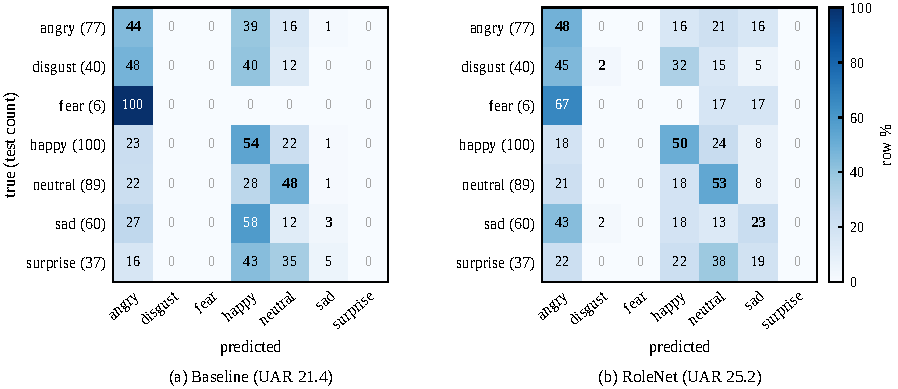
\includegraphics[width=\linewidth]{confusion_test.pdf}
\caption{Ma trận nhầm lẫn chuẩn hóa theo hàng của mô hình gốc và \model{} trên tập kiểm tra (ensemble các seed). Nhãn hàng ghi số MCIS kiểm tra của mỗi lớp}
\label{fig:confusion}
\end{figure}

\begin{figure}[!htb]
\centering
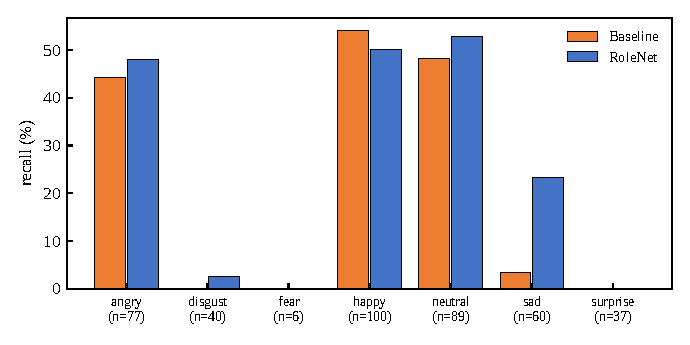
\includegraphics[width=0.8\linewidth]{recall_test.pdf}
\caption{Độ nhạy theo từng lớp trên tập kiểm tra}
\label{fig:recall}
\end{figure}

Hình~\ref{fig:confusion} và Hình~\ref{fig:recall} so sánh lỗi của hai mô hình. Mô hình gốc nhầm lẫn cực tính: nó dự đoán \emph{happy} cho 58\% các phản hồi \emph{sad} và chỉ nhận ra 3\% số đó. \model{} giảm nhầm lẫn này xuống 18\% và nâng độ nhạy của \emph{sad} lên 23\%, trong khi giữ \emph{angry}, \emph{happy} và \emph{neutral} ở mức tương đương. Không mô hình nào dự đoán đúng \emph{fear} hay \emph{surprise}, và \emph{disgust} chỉ hiếm khi đúng.

\section{Kết quả trên MELD}

\begin{table}[!htb]
\centering
\caption{Kết quả trên tập kiểm tra MELD (1.341 mẫu; UAR ngẫu nhiên 14,29). TB: trung bình các seed; Ens.: ensemble các seed}
\label{tab:meld}
\begin{tabular}{lcccc}
\toprule
 & \multicolumn{2}{c}{UAR} & \multicolumn{2}{c}{WAR} \\
\cmidrule(lr){2-3}\cmidrule(lr){4-5}
Mô hình & TB & Ens. & TB & Ens. \\
\midrule
Mô hình gốc & 15,56 & 15,50 & \textbf{43,35} & \textbf{46,09} \\
\model{} & \textbf{16,72} & \textbf{16,85} & 35,84 & 39,30 \\
\bottomrule
\end{tabular}
\end{table}

Trên MELD (Bảng~\ref{tab:meld}), UAR của \model{} cao hơn một chút so với mô hình gốc, nhưng khác biệt không có ý nghĩa thống kê. Mô hình gốc có WAR cao hơn vì dự đoán \emph{neutral} cho phần lớn các mẫu (độ nhạy \emph{neutral} 93\%, mọi lớp khác bằng 0 trừ \emph{angry}), còn \model{} phân bố dự đoán rộng hơn (độ nhạy \emph{happy} 17,9\%, \emph{angry} 17,6\%). Vì \emph{neutral} chiếm 48\% tập kiểm tra MELD, WAR thưởng cho việc dồn về lớp đông, điều mà UAR phạt. Cả hai mô hình đều gần mức ngẫu nhiên, cho thấy dự đoán cảm xúc trên MELD khi không biết người nói là rất khó.

\section{Phân tích loại bỏ thành phần}

\begin{table}[!htb]
\centering
\caption{Phân tích loại bỏ thành phần trên dữ liệu phát triển. Mọi biến thể được huấn luyện lại với cùng fold và seed; các biến thể đến từ ba lần chạy, trong đó mô hình đầy đủ đạt từ 25,92 đến 26,24 (bảng ghi giá trị cao nhất)}
\label{tab:ablation}
\begin{tabular}{lc}
\toprule
Biến thể & UAR \\
\midrule
\model{} & \textbf{26,24} \\
\midrule
\quad bỏ token người nghe & 24,20 \\
\quad bỏ ngữ cảnh clip I--II & 24,11 \\
\quad gộp mọi khuôn mặt theo clip (không có vai trò) & 25,80 \\
\midrule
\quad bỏ token người nghe ở clip III & 25,00 \\
\quad bỏ token người nói & 25,66 \\
\quad bỏ token những người còn lại & 24,64 \\
\quad bỏ token người nghe và những người còn lại & 23,22 \\
\quad bỏ token người nói, lời nói và bối cảnh & 23,10 \\
\midrule
\quad bỏ toàn bộ token khuôn mặt & 22,03 \\
\quad bỏ token lời nói và bối cảnh & 25,01 \\
\quad bỏ đầu dự đoán phụ và modality dropout & 25,15 \\
\quad đường xử lý riêng cho từng vai trò, cộng lại & 23,78 \\
\quad đường xử lý riêng cho từng vai trò, có tương tác & 24,60 \\
\bottomrule
\end{tabular}
\end{table}

Trong Bảng~\ref{tab:ablation}, mọi biến thể đều thấp hơn mô hình đầy đủ, dù một số khác biệt nhỏ. Cần lưu ý rằng các lần chạy lặp lại của cùng một mô hình với ba seed dao động khoảng $\pm0{,}4$ đến $0{,}6$ điểm UAR, nên các khác biệt dưới khoảng 1 điểm cần nhiều seed hơn mới kết luận được. Vì vậy các kết luận quan trọng dưới đây đều được kiểm tra lại với 10 seed.

\textbf{Khuôn mặt là nguồn thông tin quan trọng nhất.} Bỏ toàn bộ token khuôn mặt làm UAR giảm xuống 22,03.

\textbf{Trong các khuôn mặt, người nghe đóng góp nhiều nhất.} Chỉ bỏ token của người nghe làm UAR giảm từ 26,24 xuống 24,20; với 10 seed, mức giảm là 2,04 điểm (khoảng tin cậy [+0,21; +3,46]), xảy ra ở cả năm fold. Mức giảm tập trung ở các MCIS có người nghe xuất hiện trong clip III (+2,80) so với các MCIS không có (+0,54).

\textbf{Ngữ cảnh trước đó quan trọng tương đương.} Chỉ giữ clip III cho 24,11 (mức giảm 2,13, khoảng tin cậy [+0,20; +4,08]); phần lớn mức giảm đến từ clip II.

\textbf{Hai loại bằng chứng bổ sung cho nhau.} Một mô hình chỉ giữ khuôn mặt của người nói cùng token lời nói và bối cảnh, tức kiểu tiếp cận quanh người nói, đạt 23,22; chỉ dùng khuôn mặt của người nghe và những người còn lại đạt 23,10. Cả hai đều thấp hơn nhiều so với khi kết hợp.

\textbf{Xử lý đồng thời các token có ích.} Tách thành các đường xử lý riêng cho từng vai trò rồi cộng lại chỉ đạt 23,78 (thấp hơn 2,14 điểm, khoảng tin cậy [+0,29; +3,79]); thêm một số hạng tương tác chỉ lấy lại một phần.

\textbf{Việc tách khuôn mặt theo vai trò chưa được chứng minh là cần thiết.} Gộp mọi khuôn mặt của một clip thành một token (không có A/L/O) đạt 25,80; với 10 seed, khác biệt là +0,44 với khoảng tin cậy [$-1{,}21$; $+2{,}16$], không có ý nghĩa. Điều này khớp với việc bỏ vector nhúng vai trò cũng không làm giảm kết quả. Phiên bản gộp vẫn nhìn thấy khuôn mặt của người nghe, chỉ là trộn với người khác; nên điều quan trọng là có nét mặt của người nghe trong đầu vào, còn việc gắn nhãn vai trò cho nó thì chưa chắc. Hình~\ref{fig:cvroles} so sánh ma trận nhầm lẫn của hai phiên bản. Mục~\ref{sec:g47} trình bày một thực nghiệm kiểm soát chặt hơn cho câu hỏi này.

\begin{figure}[!htb]
\centering
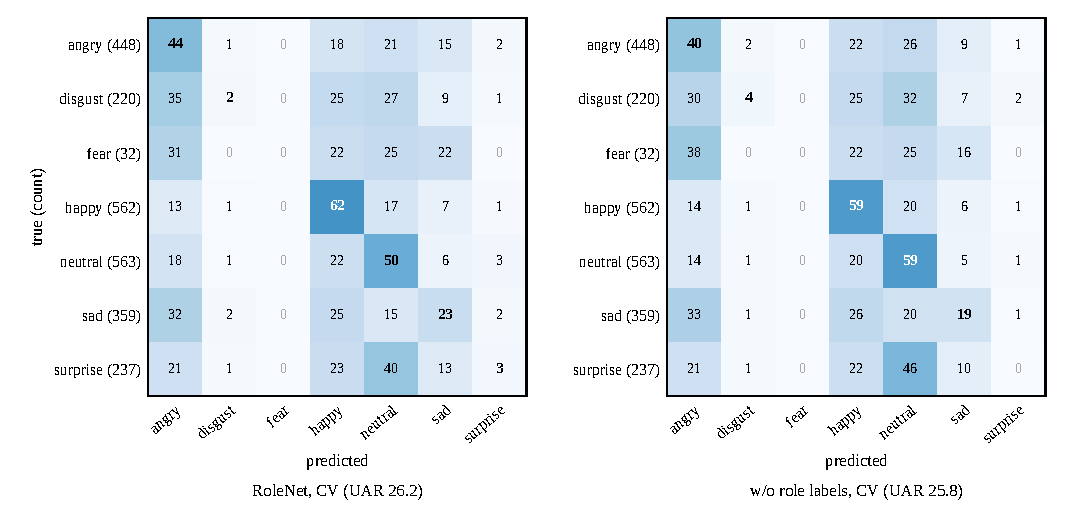
\includegraphics[width=\linewidth]{confusion_cv_roles.pdf}
\caption{Ma trận nhầm lẫn trên dữ liệu phát triển của \model{} (trái) và phiên bản gộp khuôn mặt theo clip, không có vai trò (phải)}
\label{fig:cvroles}
\end{figure}

\section{Người nghe đại diện và người phản hồi thật}
\label{sec:proxy}

Câu hỏi tiếp theo là liệu mô hình có cần biết chính xác ai sẽ phản hồi không. Một phiên bản oracle thay người nghe bằng người phản hồi thật: B được xác định là khuôn mặt chiếm ưu thế trong clip IV, rồi đối chiếu với một danh tính của clip I--III, điều này làm được với 88\% số MCIS. Phiên bản này dùng clip IV nên chỉ phục vụ phân tích. Trong số các MCIS mà quy tắc gán được người nghe, người nghe trùng với người phản hồi đã đối chiếu ở 68\%.

\begin{table}[!htb]
\centering
\caption{UAR khi dùng người nghe đại diện (không cần danh tính) và khi dùng người phản hồi thật (oracle, dùng clip IV). "Người nghe $\neq$ B": quy tắc chọn người khác hoặc không chọn ai}
\label{tab:proxy}
\begin{tabular}{lrcc}
\toprule
Nhóm mẫu (dữ liệu phát triển) & Số mẫu & Đại diện & Oracle \\
\midrule
Toàn bộ & 2.421 & 26,24 & 26,20 \\
B xuất hiện trong clip I--III & 2.107 & 26,98 & 26,90 \\
\quad người nghe $\neq$ B & 390 & 28,33 & 28,15 \\
B không xuất hiện trong clip I--III & 314 & 21,20 & 21,29 \\
\bottomrule
\end{tabular}
\end{table}

Bảng~\ref{tab:proxy} không cho thấy khác biệt đo được giữa người nghe đại diện và người phản hồi thật (toàn bộ: $-0{,}04$, khoảng tin cậy [$-1{,}50$; $+1{,}85$]), kể cả trên 390 MCIS mà quy tắc chọn sai người. Kết quả này gợi ý rằng mô hình dựa vào những gì các khuôn mặt nhìn thấy được biểu hiện, và trên Hi-EF một cách chọn bằng chứng không cần danh tính là đủ. Các MCIS mà B không xuất hiện có UAR thấp hơn rõ rệt, phù hợp với việc người phản hồi là nguồn thông tin chính.

\subsection{Phân nhóm theo độ tin cậy của việc đối chiếu}

Phép đối chiếu B với các danh tính của clip I--III có thể sai. Để kiểm tra, một phân tích bổ sung (G48) chia lại các MCIS phát triển thành bốn nhóm theo độ tin cậy: B trùng người nghe (990 MCIS), B có mặt nhưng khác người nghe (1.114), B không xuất hiện (225), và đối chiếu không chắc chắn (92). Trong nhóm "B có mặt nhưng khác người nghe", B chỉ xuất hiện trong clip III ở 19,3\% số mẫu; phần lớn còn lại B chỉ có mặt ở clip I--II, nơi quy tắc chọn người nghe (vốn chỉ xét clip III) không thể chọn được B. Nhóm đáng chú ý nhất để đánh giá giá trị của việc biết chính xác B là khoảng 215 MCIS mà B có mặt trong clip III nhưng quy tắc chọn người khác.

\choketqua{G48 -- UAR của người nghe đại diện, oracle và phiên bản không có người nghe trên từng nhóm; kết quả kiểm tra thủ công 24 mẫu}

\section{Nguồn gốc của phần cải thiện}

Mục này tách phần cải thiện so với mô hình gốc thành hai câu hỏi: nó đến từ đặc trưng tốt hơn hay từ cách tổ chức bằng chứng, và nó có phụ thuộc vào những khung hình sát lượt nói cần dự đoán không. Mọi mô hình trong Bảng~\ref{tab:origin} được huấn luyện trong cùng một lần chạy, cùng fold và cùng seed.

\begin{table}[!htb]
\centering
\caption{Nguồn gốc của phần cải thiện so với mô hình gốc (dữ liệu phát triển). Mô hình gốc dùng đặc trưng của \model{} là kiến trúc của \citet{wang2026hief} được cung cấp đặc trưng khuôn mặt, đồng bộ miệng -- âm thanh và giọng nói của \model{}, gộp theo clip. Trong các biến thể cắt clip III, chỉ \model{} bị mất phần cuối clip; các mô hình gốc vẫn thấy toàn bộ clip}
\label{tab:origin}
\begin{tabular}{lcc}
\toprule
Mô hình & UAR & WAR \\
\midrule
Mô hình gốc, đặc trưng gốc & 21,27 & 31,68 \\
Mô hình gốc, đặc trưng của \model{} & 23,25 & 32,71 \\
\midrule
\model{} & \textbf{26,62} & \textbf{37,92} \\
\quad chỉ token người nghe của clip I/II & 25,15 & 36,56 \\
\quad chỉ token người nghe của clip III & 24,86 & 35,98 \\
\quad không có token người nghe & 24,04 & 35,23 \\
\midrule
\model{}, giữ 80\% đầu của clip III & 25,73 & 37,01 \\
\model{}, giữ 60\% đầu của clip III & 25,08 & 36,14 \\
\bottomrule
\end{tabular}
\end{table}

\textbf{Đặc trưng hay cách tổ chức?} Cung cấp cho kiến trúc gốc các đặc trưng của \model{}, gộp theo clip như thông thường, nâng UAR từ 21,27 lên 23,25 (khác biệt +1,98, không có ý nghĩa). \model{} vẫn hơn mô hình này 3,37 điểm (khoảng tin cậy [+0,68; +5,09]) ở cả năm fold. Như vậy đặc trưng phong phú hơn chỉ giải thích một phần phần cải thiện. Phần còn lại gắn với token người nghe: khi bỏ chúng, \model{} không còn phân biệt được với mô hình gốc dùng cùng đặc trưng (+0,79). Token người nghe của clip I/II hoặc của clip III riêng lẻ mỗi loại lấy lại một phần khoảng cách (lần lượt +1,12 và +0,83 so với khi không có người nghe, đều chưa có ý nghĩa), và chỉ khi có cả hai mô hình mới trở lại mức đầy đủ (+2,58, có ý nghĩa).

\textbf{Dự đoán hay nhận ra phản ứng sớm?} Khoảng một nửa số khung hình có người nghe nằm ở 20\% cuối của clip III, rất gần lượt nói cần dự đoán. Nếu mô hình chỉ nhận ra phản ứng đã bắt đầu của người phản hồi, đó gần với nhận diện hơn là dự đoán. Để kiểm tra, \model{} được huấn luyện lại khi cắt bỏ phần cuối của clip III: khuôn mặt sau điểm cắt bị loại trước khi gán vai trò, và token bối cảnh chỉ dùng các khung hình còn lại; các mô hình gốc vẫn thấy toàn bộ clip. Khi giữ 80\% hoặc 60\% clip III, \model{} vẫn hơn mô hình gốc 4,46 và 3,81 điểm, và hơn mô hình gốc dùng cùng đặc trưng 2,48 và 1,83 điểm, tất cả đều có ý nghĩa, dù khoảng cách với mô hình gốc dùng cùng đặc trưng là nhỏ.

Phần đóng góp riêng của người nghe giảm khi cắt. Với quy tắc chọn người nghe thông thường, đóng góp này giảm từ 2,58 xuống 1,15 rồi $-0{,}13$; nhưng ở đây việc cắt còn làm mất luôn danh tính người nghe trong nhiều mẫu. Khi cố định người nghe là người phản hồi thật (oracle như Mục~\ref{sec:proxy}), để việc cắt chỉ bỏ khung hình chứ không bỏ danh tính, đóng góp giảm từ 2,85 xuống 1,57 rồi 1,21: khoảng một nửa còn lại khi không có các khung hình cuối, tương đương giá trị của token người nghe ở clip I/II. Không nửa nào có ý nghĩa thống kê khi đứng riêng. Kết quả gợi ý rằng mô hình dựa vào cả những lần xuất hiện trước đó của người phản hồi lẫn phản ứng của họ ở cuối lượt hiện tại, với mức độ tương đương nhau.

\section{Bộ mã hóa có cần thêm cấu trúc?}
\label{sec:structure}

Nhiều ý tưởng cải tiến tự nhiên là thêm cấu trúc vào bộ mã hóa: mã hóa thứ tự thời gian, quan hệ giữa các người, hay tách riêng các nhóm bằng chứng. Bảng~\ref{tab:structure} tổng hợp các thử nghiệm theo hướng này, đánh giá bằng NLL sau temperature scaling vì các hiệu ứng mong đợi nhỏ.

\begin{table}[!htb]
\centering
\caption{Các biến thể cấu trúc của \model{}: NLL trên dữ liệu giữ lại sau temperature scaling, so với \model{} (dương = kém hơn). Nhóm EMAP: người nghe, lịch sử (các token khác của clip I--II) và sự kiện hiện tại (các token khác của clip III)}
\label{tab:structure}
\begin{tabular}{lc}
\toprule
Thay đổi so với \model{} & $\Delta$NLL \\
\midrule
Bỏ thứ tự giữa clip I và II & $+0{,}006$ \\
Bỏ thứ tự giữa cả ba clip & $+0{,}008$ \\
Thêm độ lệch chú ý theo thời gian, người và loại bằng chứng & $+0{,}001$ \\
Xấp xỉ cộng tính tốt nhất (EMAP) & $+0{,}011$ \\
\bottomrule
\end{tabular}
\end{table}

Làm cho bộ mã hóa bất biến hoàn toàn với thứ tự của clip I và II, hoặc của cả ba clip (đã kiểm tra bằng số: thay đổi logit lớn nhất là $1{,}4\cdot10^{-6}$), không làm kết quả kém đi có ý nghĩa. Các độ lệch chú ý theo thời gian, người và loại bằng chứng được học nhưng không mang lại cải thiện đo được; các cách đọc kết quả khác (trung bình các token, đọc token người nghe, truy vấn chỉ đọc, ba truy vấn) cũng vậy.

Tuy nhiên, phân tích EMAP \cite{hessel2020emap} cho thấy bộ mã hóa sau huấn luyện \emph{có} dùng tương tác không cộng tính. EMAP thay mô hình bằng xấp xỉ cộng tính tốt nhất theo ba nhóm token (người nghe, lịch sử, sự kiện hiện tại); NLL tăng 0,011 (có ý nghĩa), và mỗi nhóm đều tương tác với phần còn lại. Các tương tác này khiêm tốn, chiếm khoảng 5\% phương sai của logit, và không liên quan đến lời thoại: tách cộng tính giữa văn bản và mọi thứ khác không làm mất gì đo được. Kết luận chung: tự chú ý đồng thời trên các token đã đủ, các cấu trúc tường minh đã thử không mang lại thêm lợi ích.

\section{Phân tích lỗi}

\subsection{Lặp lại cảm xúc của người nói}

\begin{figure}[!htb]
\centering
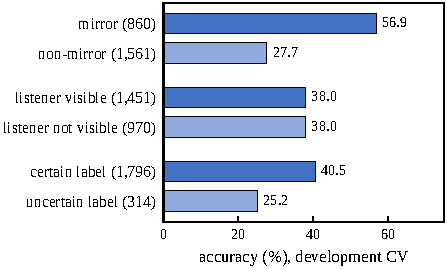
\includegraphics[width=0.62\linewidth]{errors_by_group_cv.pdf}
\caption{Độ chính xác của \model{} theo nhóm mẫu trên dữ liệu phát triển}
\label{fig:groups}
\end{figure}

Hơn một nửa số dự đoán đúng là các trường hợp mirroring. Trên các MCIS mà B lặp lại cảm xúc của A, \model{} đúng 56,9\%, nhưng chỉ 27,7\% ở các trường hợp còn lại, nơi nó vẫn dự đoán cảm xúc của A trong 29\% số mẫu (Hình~\ref{fig:groups}). Token người nghe giúp chủ yếu ở các trường hợp mirroring. Việc B có lặp lại A hay không là dự đoán được một phần (AUC 0,70), nhưng B sẽ chuyển sang cảm xúc nào thì gần như không: trên các trường hợp không lặp lại, độ nhạy của \emph{disgust} là 1,6\%, \emph{surprise} 2,8\% và \emph{fear} 0\%.

\subsection{Giữ cảm xúc của chính mình}

\begin{table}[!htb]
\centering
\caption{Độ chính xác (\%) theo việc B giữ hay đổi cảm xúc của chính mình so với lượt nói trước của B (dữ liệu phát triển, cùng lần chạy với Bảng~\ref{tab:origin}). "Đặc trưng \model{}": mô hình gốc dùng đặc trưng của \model{}}
\label{tab:keep}
\begin{tabular}{lrccc}
\toprule
Nhóm mẫu & Số mẫu & Mô hình gốc & Đặc trưng \model{} & \model{} \\
\midrule
Toàn bộ & 2.421 & 31,7 & 32,7 & \textbf{37,9} \\
B giữ cảm xúc & 320 & 46,3 & 45,6 & \textbf{56,6} \\
\quad và trùng với A & 145 & 55,9 & 53,8 & \textbf{71,0} \\
\quad và khác A & 175 & 38,3 & 38,9 & \textbf{44,6} \\
B đổi cảm xúc & 334 & 27,0 & 27,0 & \textbf{27,8} \\
\quad sang cảm xúc của A & 90 & 41,1 & 36,7 & \textbf{43,3} \\
\quad sang cảm xúc khác A & 244 & 21,7 & \textbf{23,4} & 22,1 \\
Không biết cảm xúc trước của B & 1.767 & 29,9 & 31,5 & \textbf{36,5} \\
\bottomrule
\end{tabular}
\end{table}

Quán tính cảm xúc cho một bức tranh tương tự (Bảng~\ref{tab:keep}). Ở 27\% số MCIS, B đã nói ở clip I hoặc II với một nhãn cảm xúc (B được xác định qua giọng nói trong clip IV, chỉ để phân tích), và B giữ cảm xúc đó trong 48,9\% trường hợp. Lợi thế của \model{} so với mô hình gốc lớn nhất ở các trường hợp B giữ cảm xúc: đúng 56,6\% so với 46,3\%, và 71,0\% so với 55,9\% khi cảm xúc được giữ cũng trùng với A. Khi B chuyển sang cảm xúc khác, mọi mô hình chỉ đúng khoảng 27\%, và khoảng 22\% khi cảm xúc mới cũng khác của A. Đây là phép so sánh mô tả: với 320 mẫu, khoảng tin cậy của khác biệt trên nhóm "giữ cảm xúc" vẫn chạm 0.

\subsection{Nhãn không chắc chắn và sự có mặt của người nghe}

Khi người chú thích đánh dấu nhãn của B là không chắc chắn, độ chính xác giảm từ 40,5\% xuống 25,2\%, phù hợp với việc sự mơ hồ của nhãn giới hạn mức mà bất kỳ mô hình nào có thể đạt. Độ chính xác không phụ thuộc vào việc người nghe có xuất hiện trong clip III hay không (38,0\% ở cả hai nhóm), phù hợp với việc mô hình dựa vào ngữ cảnh và người nói khi không thấy người nghe.

\subsection{Giới hạn nằm ở việc nhận diện}

Hai phân tích oracle gợi ý rằng thông tin còn thiếu chủ yếu là vấn đề nhận diện. Khi thêm cảm xúc thật của A trong clip III vào đầu ra của \model{}, UAR của một mô hình tuyến tính trên các đầu ra này tăng từ 24,73 lên 27,51 và NLL giảm 0,036; nhưng khi cảm xúc của A được ước lượng bằng một bộ nhận diện từ clip III, phần tăng biến mất. Trên các MCIS biết lượt nói trước của B, chỉ cần sao chép cảm xúc trước đó của B đã đạt 39,18 UAR, so với 27,39 của \model{}, và thêm đầu ra của \model{} vào nhãn đó không cải thiện thêm đáng kể (+1,44, khoảng tin cậy [$-4{,}75$; $+8{,}39$]). Như vậy tín hiệu còn thiếu nằm ở trạng thái cảm xúc hiện tại của những người tham gia, mà các bộ trích xuất đặc trưng cố định nhận diện kém; các cách kết hợp khác nhau của cùng các token đã thử không lấy lại được nó. Chương 5 trình bày các nỗ lực nhằm cải thiện việc nhận diện này.

\section{Kiểm soát vai trò của việc tổ chức theo người}
\label{sec:g47}

Kết quả ở Mục 4.4 cho thấy gộp khuôn mặt theo clip chỉ kém \model{} 0,44 điểm, không có ý nghĩa. Tuy nhiên phép so sánh đó chưa hoàn toàn tương đương: phiên bản gộp không có đầu dự đoán phụ cho cảm xúc của A, vì không có token riêng của A. Để làm rõ phần đóng góp nào đến từ việc giữ bằng chứng riêng theo người, từ việc gán vai trò và từ việc chọn người nghe, thực nghiệm G47 huấn luyện lại trong cùng một lần chạy (10 seed $\times$ 5 fold) các biến thể sau:

\begin{itemize}
	\item token theo người so với gộp theo clip, cả khi có và khi không có các đầu dự đoán phụ; phiên bản gộp cũng gộp độ đồng bộ miệng -- âm thanh theo clip, để không còn thông tin vai trò;
	\item bỏ vector nhúng vai trò; và hoán đổi A với L ở một nửa ngẫu nhiên các mẫu, nhất quán qua cả ba clip, để phá thông tin vai trò mà vẫn giữ riêng từng người;
	\item chọn người nghe ngẫu nhiên trong số những người không nói ở clip III (ba lần chọn khác nhau), so với người nghe theo quy tắc và với phiên bản không có người nghe, đánh giá chủ yếu trên các mẫu có ít nhất hai ứng viên.
\end{itemize}

Quy tắc đọc kết quả được cố định trước: việc tổ chức theo người được coi là có lợi nếu cận dưới khoảng tin cậy của khác biệt dương ở cả cặp có và không có đầu dự đoán phụ; việc gán vai trò mang thông tin nếu \model{} hơn phiên bản hoán đổi một cách có ý nghĩa; và việc chọn người nghe có giá trị nếu \model{} hơn phiên bản chọn ngẫu nhiên trên các mẫu có ít nhất hai ứng viên.

\choketqua{G47 -- bảng UAR/WAR (trung bình $\pm$ độ lệch chuẩn theo seed), khác biệt theo cặp, khoảng tin cậy và kết luận theo ba quy tắc trên}

\newpage
\clearpage
\phantomsection
\chapter[CÁC HƯỚNG ĐÃ THỬ NHƯNG KHÔNG THÀNH CÔNG]{Các hướng đã thử nhưng không thành công}
\label{chap:negative}

Bên cạnh \model{}, trong quá trình thực tập nhiều hướng cải tiến khác đã được đề xuất và kiểm tra. Phần lớn không mang lại cải thiện. Chương này ghi lại các hướng đó vì hai lý do: chúng giúp khoanh vùng chỗ thực sự là nút thắt của bài toán, và một kết quả âm được kiểm tra cẩn thận cũng là thông tin có giá trị cho người nghiên cứu sau. Mỗi hướng được trình bày theo cùng một khuôn: giả thuyết, cách kiểm tra, kết quả và lý do dừng. Tất cả các thực nghiệm dưới đây dùng dữ liệu phát triển, trừ khi ghi rõ. Bảng~\ref{tab:negative} tóm tắt các hướng chính.

\begin{table}[!htb]
\centering
\caption{Tóm tắt các hướng đã thử nhưng không thành công}
\label{tab:negative}
{\fontsize{11}{13}\selectfont
\begin{tabular}{>{\raggedright}p{4.2cm}>{\raggedright}p{2.2cm}>{\raggedright\arraybackslash}p{8.2cm}}
\toprule
Hướng & Thực nghiệm & Kết quả chính \\
\midrule
Nhận diện rồi chuyển trạng thái & G1--G5 & Ngang mô hình dự đoán trực tiếp trên tập kiểm định \\
Gắn vai trò người nói cho lời thoại & G9 & +0,11, không ý nghĩa; con trỏ hoàn hảo cũng không giúp \\
Động lực học cảm xúc liên tục & G15--G17 & Không thấy cảm xúc phai dần theo thời gian \\
Thay đổi cách gộp và cấu trúc & G12, G28--G33 & Không cải thiện đo được \\
Đánh giá tình huống bằng mô hình ngôn ngữ & G24 & Không giúp dự đoán hướng phản ứng \\
Cân bằng lớp khi huấn luyện & G36, G38 & Chỉ dịch chuyển độ nhạy giữa các lớp \\
Đặc trưng cảm xúc chuyên biệt & G45 & Nhận diện tăng ít, dự đoán không đổi \\
Dùng cảm xúc trước của B & Mô phỏng & Chỉ có lợi khi nhận diện gần hoàn hảo \\
Học từ khuôn mặt tương lai & G46a & \choketqua{G46a} \\
\bottomrule
\end{tabular}}
\end{table}

\section{Nhận diện rồi chuyển trạng thái}

\textbf{Giả thuyết.} Nếu biết cảm xúc thật của A ở clip III, một mô hình đơn giản đã đạt khoảng 28 UAR, cao hơn các mô hình lúc đó. Vì vậy có thể tách bài toán thành hai bước: nhận diện cảm xúc của các lượt trước, rồi dự đoán cảm xúc của B từ "quỹ đạo" cảm xúc đó.

\textbf{Kiểm tra.} Một bộ nhận diện cảm xúc cho từng clip được huấn luyện chéo trên các tập phim huấn luyện; xác suất cảm xúc, cực tính, độ tin cậy và entropy của từng clip I--III tạo thành quỹ đạo làm đầu vào cho bộ dự đoán. Bộ nhận diện dùng đặc trưng CLIP và AudioCLIP chỉ đạt khoảng 23 UAR khi nhận diện cảm xúc của A.

\textbf{Kết quả.} Khi chọn mô hình trên tập kiểm định theo đúng quy trình báo cáo, bộ dự đoán dùng quỹ đạo ngang bằng một mô hình dự đoán trực tiếp từ đặc trưng clip (26,23 so với 25,77 UAR trung bình theo seed; khác biệt của ensemble $-0{,}62$, khoảng tin cậy [$-2{,}98$; $+2{,}52$]).

\textbf{Lý do dừng.} Bước nhận diện quá yếu, nên lợi ích của việc biết cảm xúc trước đó không truyền được sang bước dự đoán. Bài học này lặp lại ở nhiều hướng khác bên dưới.

\section{Gắn vai trò người nói cho lời thoại}

\textbf{Giả thuyết.} Lượt nói trước của chính B dự đoán cảm xúc tiếp theo của B tốt nhất: nhãn ở clip II trùng với nhãn của B trong 50,6\% trường hợp nếu B là người nói clip II, so với khoảng 35\% nếu đó là A. Vì vậy gắn cho mỗi câu thoại ở clip I/II một trọng số "do A nói / do B nói / do người khác nói", và thêm một token cho lượt nói trước của B, có thể giúp mô hình.

\textbf{Kiểm tra.} Phiên bản \model{}+ (G9) dùng một con trỏ dự đoán câu nào do B nói từ các tín hiệu trong clip I--III (AUC 0,82). Nhãn huấn luyện của con trỏ lấy từ giọng nói ở clip IV, chỉ khi huấn luyện. Một phiên bản oracle dùng con trỏ hoàn hảo để đo mức trần.

\textbf{Kết quả.} \model{}+ chỉ hơn \model{} 0,11 điểm UAR (khoảng tin cậy [$-2{,}23$; $+2{,}03$]), dương ở 2/5 fold. Con trỏ hoàn hảo cũng không giúp ($-0{,}64$).

\textbf{Lý do dừng.} Ngay cả khi biết chính xác B đã nói câu nào, mô hình vẫn phải tự nhận diện cảm xúc của câu đó từ đặc trưng, và đó mới là khâu yếu.

\section{Động lực học cảm xúc liên tục}

\textbf{Giả thuyết.} Trạng thái cảm xúc của B có thể được mô hình hóa như một quá trình liên tục theo thời gian, ví dụ quá trình Ornstein--Uhlenbeck: trạng thái phai dần về mức nền và bị kéo về phía cảm xúc của người đối diện. Nếu đúng, các quan sát gần lượt nói cần dự đoán sẽ mang nhiều thông tin hơn, và mức độ phụ thuộc vào khoảng thời gian trôi qua.

\textbf{Kiểm tra.} Một chuỗi phép kiểm tra (G15--G17) so sánh lượng thông tin (tính bằng bit) về nhãn của B mà khuôn mặt của B mang lại khi được quan sát gần (clip III) và xa (clip I/II), trong khi giữ cố định loại quan sát (đang nghe hay đang nói) và số khung hình.

\textbf{Kết quả.} Quan sát gần mang nhiều thông tin hơn quan sát xa khoảng bốn lần (+0,079 bit, có ý nghĩa). Nhưng khi giữ cố định loại quan sát, khuôn mặt ở clip II không mang nhiều thông tin hơn ở clip I ($-0{,}017$ bit, khoảng tin cậy [$-0{,}115$; $+0{,}078$]), và quan sát lúc nghe không hơn lúc nói. Phần lợi thế của quan sát gần chủ yếu đến từ việc các quan sát xa thường là lúc B đang nói, chứ không phải từ thời gian trôi qua. Đóng góp của người nghe cũng không phụ thuộc vào khoảng cách thời gian đến clip IV (hệ số tương quan Spearman +0,005).

\textbf{Lý do dừng.} Ở thang thời gian của Hi-EF (vài giây mỗi clip), dữ liệu không ủng hộ mô hình suy giảm liên tục; trạng thái thay đổi theo từng bước, theo lượt nói.

\section{Thay đổi cách gộp và cấu trúc của mô hình}

Một nhóm thử nghiệm giữ nguyên bằng chứng nhưng thay đổi cách mô hình xử lý nó.
\begin{itemize}
	\item \textbf{Đường xử lý riêng cho từng vai trò} (G12): kém hơn \model{} 2,14 điểm; thêm tương tác chỉ lấy lại một phần (Bảng~\ref{tab:ablation}).
	\item \textbf{Huấn luyện với người nghe bị che ngẫu nhiên} (G28), để mô hình quen với việc thiếu người nghe: không cải thiện có ý nghĩa ($\Delta$NLL +0,0037, khoảng tin cậy [$-0{,}0066$; $+0{,}0153$]).
	\item \textbf{Gộp khung hình có điều kiện theo ngữ cảnh} (G29), để ngữ cảnh chọn khung hình khuôn mặt nào được chú ý: không phân biệt được với cách gộp hiện tại.
	\item \textbf{Hỗn hợp "lặp lại A / phần còn lại"} (G31): một phiên bản tuyến tính còn kém hơn một chút so với cộng logit thông thường, và cổng hỗn hợp thu về gần 0.
	\item \textbf{Thứ tự clip và độ lệch chú ý theo quan hệ} (G33): không cải thiện (Bảng~\ref{tab:structure}).
\end{itemize}
Các kết quả này cùng chỉ ra rằng, với cùng một bộ bằng chứng, cách kết hợp hiện tại đã khai thác gần hết thông tin; các cấu trúc tường minh không bổ sung được gì đo được.

\section{Đánh giá tình huống bằng mô hình ngôn ngữ}

\textbf{Giả thuyết.} Theo lý thuyết đánh giá (appraisal), phản ứng cảm xúc phụ thuộc vào cách một người đánh giá tình huống. Một mô hình ngôn ngữ lớn đọc phụ đề của clip I--III có thể ước lượng các chiều đánh giá này và giúp dự đoán hướng phản ứng tiêu cực của B.

\textbf{Kết quả} (G24). Thêm các đánh giá do mô hình ngôn ngữ sinh ra không cải thiện việc phân biệt hướng phản ứng (+0,002, khoảng tin cậy [$-0{,}005$; $+0{,}010$]). Các đánh giá gần như suy biến: chúng chỉ nắm được chiều tích cực -- tiêu cực, không phân biệt được các cảm xúc tiêu cực ngay cả của chính A trong văn bản.

\section{Cân bằng lớp khi huấn luyện}

\textbf{Giả thuyết.} \model{} gần như không bao giờ dự đoán đúng các lớp hiếm (\emph{fear}, \emph{surprise}, \emph{disgust}). Lấy mẫu lại theo tần suất lớp khi huấn luyện có thể cải thiện các lớp này.

\textbf{Kết quả} (G36, G38). Lấy mẫu theo căn bậc hai nghịch đảo tần suất tăng UAR trên dữ liệu phát triển từ 26,10 lên 26,95 (+0,86, không ý nghĩa). Theo quy tắc cố định trước, biến thể này được đọc trên tập kiểm tra một lần thứ hai (được ghi rõ là một lần truy cập bổ sung): UAR 25,64 so với 25,24 của \model{} (+0,40, không ý nghĩa), với \emph{disgust} tăng từ 2,5\% lên 22,5\% nhưng \emph{angry} giảm từ 48,1\% xuống 20,8\%, và \emph{fear} vẫn bằng 0. Các mức lấy mẫu nhẹ hơn (G38) không có mức nào đáp ứng quy tắc "không làm lớp nào giảm quá 5 điểm".

\textbf{Lý do dừng.} Lấy mẫu lại chỉ phân phối lại độ nhạy giữa \emph{angry} và các lớp hiếm trong khi UAR gần như không đổi. Mô hình cuối cùng vẫn là \model{} đã đăng ký trước.

\section{Đặc trưng cảm xúc chuyên biệt}

\textbf{Giả thuyết.} Token lời nói của \model{} dùng CLIP, AudioCLIP và ECAPA, không mô hình nào chuyên về cảm xúc. Các mô hình cảm xúc có sẵn có thể giúp nhận diện trạng thái của người tham gia tốt hơn.

\textbf{Kiểm tra} (G45). Hai mô hình cố định, không huấn luyện trên MELD, được thêm vào: mô hình cảm xúc giọng nói wav2vec2 của \citet{wagner2023dawn} (huấn luyện trên MSP-Podcast) và mô hình văn bản RoBERTa huấn luyện trên GoEmotions \cite{demszky2020goemotions}. Hai bộ phân loại tuyến tính so sánh đặc trưng hiện có với đặc trưng hiện có cộng đặc trưng cảm xúc, cho việc nhận diện cảm xúc của từng clip và cho việc dự đoán. Quy tắc cố định trước: nhận diện lượt nói trước của B phải tăng ít nhất 5 điểm UAR với cận dưới dương.

\textbf{Kết quả.} Nhận diện tăng khoảng 1,5--2 điểm, chỉ có ý nghĩa ở clip III (+2,07). Trên lượt nói trước của B, UAR tăng từ 27,19 lên 29,67 (+2,47, khoảng tin cậy [$-1{,}27$; $+5{,}58$]), không đạt ngưỡng. Dự đoán tuyến tính gần như không đổi (18,86 so với 18,92). Theo quy tắc, hướng này dừng lại.

\section{Dùng cảm xúc trước của người phản hồi}

\textbf{Giả thuyết.} Vì sao chép cảm xúc trước của B đạt 39,18 UAR (Bảng~\ref{tab:copy}), có thể thêm một "đường tắt" đưa cảm xúc đã nhận diện của B vào bước dự đoán.

\textbf{Kiểm tra.} Một mô phỏng trên 654 MCIS biết cảm xúc trước của B thêm cảm xúc đó, với các mức độ chính xác nhận diện khác nhau, vào đầu ra của \model{}.

\textbf{Kết quả.} Khi cảm xúc trước của B được biết chính xác, UAR trên nhóm này tăng 8,15 điểm (khoảng 2,2 điểm trên toàn bộ dữ liệu). Nhưng khi độ chính xác nhận diện là 60\%, mức tăng còn $-0{,}12$; ở 31\%, xấp xỉ khả năng hiện tại của bộ nhận diện, kết quả còn kém đi 2,46 điểm. Đường tắt này chỉ có ích nếu việc nhận diện trạng thái trước đó của B tốt hơn rất nhiều so với hiện nay, và còn đòi hỏi biết lượt nói nào là của B, điều bản thân nó cũng không chắc chắn khi suy luận.

\section{Học từ khuôn mặt tương lai khi huấn luyện}

\textbf{Giả thuyết.} Mỗi MCIS chỉ có một nhãn bảy lớp, trong khi khuôn mặt của B ở clip IV, chính khoảnh khắc mà nhãn mô tả, chứa nhiều thông tin hơn. Dùng khuôn mặt này làm \emph{mục tiêu phụ chỉ khi huấn luyện} (học với thông tin đặc quyền) có thể giúp mô hình học biểu diễn tốt hơn mà không vi phạm ràng buộc không dùng clip IV khi suy luận.

\textbf{Kiểm tra} (G46a). Một phép kiểm tra tuyến tính dự đoán vector biểu cảm khuôn mặt của B ở clip IV từ clip I--III bằng hồi quy ridge, rồi thêm dự đoán đó vào bộ phân loại. Đối chứng là cùng quy trình nhưng mục tiêu bị xáo trộn giữa các mẫu. Quy tắc: mục tiêu phải mang thông tin về nhãn (kiểm tra bằng oracle), và dự đoán của nó phải tốt hơn cả đặc trưng hiện có lẫn đối chứng xáo trộn.

\choketqua{G46a -- R² của hồi quy, UAR của các biến thể và kết luận theo quy tắc}

\section{Bài học rút ra}

\begin{itemize}
	\item \textbf{Bằng chứng quan trọng hơn cấu trúc.} Những gì tạo ra khác biệt là việc có đúng nguồn thông tin trong đầu vào: khuôn mặt của người nghe và ngữ cảnh của các lượt trước. Các thay đổi về cấu trúc mô hình, cách gộp hay cách đọc kết quả đều không mang lại cải thiện đo được.
	\item \textbf{Nút thắt là nhận diện trạng thái.} Nhiều hướng thất bại vì cùng một lý do: thông tin về cảm xúc trước đó của người tham gia rất có giá trị khi biết chính xác, nhưng các bộ trích xuất hiện có không nhận diện được nó đủ tốt.
	\item \textbf{Quy tắc cố định trước giúp tránh tự đánh lừa.} Mỗi thực nghiệm đều có quy tắc đọc kết quả được viết trước khi chạy, và các khác biệt nhỏ được kiểm tra lại với nhiều seed hơn. Nhờ vậy những cải thiện "trông có vẻ" tốt nhưng nằm trong mức nhiễu không bị đưa vào mô hình cuối.
	\item \textbf{Tập kiểm tra là tài nguyên có hạn.} Mỗi lần đọc tập kiểm tra đều được ghi lại; kết quả của lần đọc thứ hai được báo cáo kèm điều kiện đó.
\end{itemize}

\newpage
\clearpage
\phantomsection
\addcontentsline{toc}{chapter}{Kết luận và hướng phát triển}
\chapter*{Kết luận và hướng phát triển}
\label{chap:conclusion}

\section*{1. Kết luận}

Báo cáo đã nghiên cứu bài toán dự đoán cảm xúc của người phản hồi trong hội thoại đa phương thức trên bộ dữ liệu Hi-EF. Từ phân tích dữ liệu, có thể rút ra rằng Hi-EF thực chất là hội thoại nhiều người, phim được dựng theo kiểu cảnh -- cảnh phản ứng, và người sẽ phản hồi thường đã xuất hiện trên màn hình với vai trò người nghe. Dựa trên đó, báo cáo đề xuất \model{}: chọn người nghe làm đại diện cho người phản hồi mà không dùng thông tin tương lai, biểu diễn mỗi người trong mỗi lượt bằng một token, và đọc tập token bằng một bộ mã hóa tập hợp nhỏ.

Các kết quả chính gồm:
\renewcommand{\labelitemi}{$-$}
\begin{itemize}
	\item Trên tập kiểm tra được khóa, đọc một lần theo kế hoạch đăng ký trước, \model{} tăng UAR từ 21,40 lên 25,24 và WAR từ 32,52 lên 36,43 so với mô hình gốc huấn luyện lại, thắng ở bảy trên tám tập phim. Chỉ số chính đã đăng ký trước (UAR sau hiệu chỉnh logit) tăng tương tự nhưng không có ý nghĩa thống kê, chủ yếu do lớp \emph{fear} chỉ có 6 mẫu kiểm tra.
	\item \model{} dùng 0,71 triệu tham số, ít hơn khoảng 40 lần so với mô hình gốc.
	\item Khuôn mặt của người nghe và ngữ cảnh của các lượt trước là hai nguồn thông tin được xác nhận, mỗi nguồn đóng góp khoảng hai điểm UAR trên dữ liệu phát triển. Phần cải thiện so với mô hình gốc không chỉ do đặc trưng tốt hơn, và vẫn còn khi bỏ phần cuối của lượt nói hiện tại.
	\item Người nghe được chọn tự động cho kết quả tương đương người phản hồi thật, và cũng tương đương một người không nói được chọn ngẫu nhiên trong clip III; gắn nhãn vai trò cho các token không tạo khác biệt đo được. Token theo người có xu hướng tốt hơn gộp theo clip khoảng một điểm UAR nhưng chưa vượt qua mức nhiễu. Các cấu trúc bổ sung đã thử cho bộ mã hóa không mang lại cải thiện đo được.
	\item Lợi thế của \model{} lớn nhất khi người phản hồi lặp lại cảm xúc của người nói hoặc giữ cảm xúc của chính mình; khi người phản hồi chuyển sang một cảm xúc mới, mọi mô hình đều gần mức đoán ngẫu nhiên.
\end{itemize}

Qua quá trình thực tập, kết luận quan trọng nhất là giới hạn hiện tại của bài toán nằm ở việc nhận diện trạng thái cảm xúc của những người tham gia, không nằm ở cách kết hợp bằng chứng. Nhiều hướng cải tiến, từ mô hình hai bước, động lực học cảm xúc, cân bằng lớp đến đặc trưng cảm xúc chuyên biệt, đều dừng lại ở cùng nút thắt này.

\section*{2. Hạn chế}

\begin{itemize}
	\item Kết luận chính dựa trên UAR thông thường, vốn được đăng ký là phân tích mô tả; chỉ số chính đã đăng ký không có ý nghĩa thống kê. Tập kiểm tra nhỏ (8 tập phim) nên khoảng tin cậy rộng.
	\item Tập kiểm tra đã từng được dùng cho các họ mô hình khác trước \model{}, và được đọc thêm một lần cho biến thể cân bằng lớp. Mọi lần truy cập được liệt kê ở Phụ lục~\ref{app:access}.
	\item Thiết kế \model{} dựa trên các phân tích trên chính dữ liệu phát triển dùng cho kiểm định chéo, nên các con số kiểm định chéo mang tính khám phá.
	\item Người phản hồi thật trong các phân tích oracle được xấp xỉ bằng khuôn mặt chiếm ưu thế trong clip IV, nên lỗi đối chiếu có thể làm mờ các so sánh. Cảm xúc trước của B chỉ biết được ở 27\% số mẫu.
	\item Văn bản và âm thanh được mã hóa bằng các mô hình đa dụng (CLIP, AudioCLIP); các encoder cảm xúc cố định chỉ cải thiện ít trong thử nghiệm tuyến tính, còn encoder được tinh chỉnh chưa được thử.
	\item Quy tắc chọn người nghe dựa vào kiểu dựng phim truyền hình, nên có thể không phù hợp với video quay bằng máy cố định. Trên MELD, cải thiện nhỏ và không có ý nghĩa.
\end{itemize}

\section*{3. Hướng phát triển}

\begin{itemize}
	\item \textbf{Nhận diện trạng thái tốt hơn.} Huấn luyện hoặc tinh chỉnh bộ nhận diện cảm xúc cho từng người trong video nhiều người, thay vì dùng các mô hình cố định huấn luyện trên dữ liệu khác.
	\item \textbf{Học với thông tin đặc quyền.} Dùng khuôn mặt của người phản hồi ở lượt cần dự đoán làm mục tiêu phụ khi huấn luyện (hướng G46a), nếu phép kiểm tra tuyến tính cho thấy tín hiệu.
	\item \textbf{Các lớp hiếm.} \emph{fear} và \emph{surprise} chủ yếu xuất hiện khi người phản hồi rời khỏi cảm xúc của người nói; cần thêm dữ liệu cho các phản ứng này hoặc cách đánh giá phù hợp hơn với lớp hiếm.
	\item \textbf{Đánh giá tổng quát hơn.} Kiểm tra quy tắc chọn người nghe và \model{} trên dữ liệu không phải phim truyền hình, nơi không có kiểu dựng cảnh -- cảnh phản ứng.
\end{itemize}

\newpage

\appendix
\chapter{Phụ lục}

\section{Siêu tham số}
\label{app:hparams}

\begin{table}[!htb]
\centering
\caption{Siêu tham số của \model{} và mô hình gốc (cố định trước khi chạy trên tập kiểm tra, không điều chỉnh theo tập kiểm tra)}
\label{tab:hparams}
{\fontsize{12}{14}\selectfont
\begin{tabular}{>{\raggedright}p{4.5cm}>{\raggedright\arraybackslash}p{10cm}}
\toprule
Lấy mẫu khuôn mặt & 4 khung hình/giây, tối đa 32 khung hình mỗi clip, tối đa 24 khung hình mỗi ô vai trò \\
Gom cụm danh tính & ArcFace, liên kết trung bình, ngưỡng cosine 0,45 \\
Đặc trưng khung hình & PCA 128 chiều của HSEmotion (khớp theo fold) + 18 đặc trưng hình học/biểu cảm \\
Giọng nói & ECAPA, cùng người nói nếu cosine $\ge$ 0,35 \\
Bộ mã hóa & 2 khối SAB pre-norm, $d = 128$, 4 đầu, FFN 512, dropout 0,2 \\
Đầu ra & LN, dropout 0,3, tuyến tính \\
Trọng số mất mát phụ & 0,3 (khuôn mặt, ngữ cảnh, A) \\
Modality dropout & ngữ cảnh 0,3, nếu không thì khuôn mặt 0,15 \\
Tối ưu & AdamW, tốc độ học $3\cdot10^{-4}$, weight decay $10^{-2}$, batch 64 \\
Lịch huấn luyện & tối đa 80 epoch, dừng sau 12 epoch không cải thiện UAR trên dữ liệu giữ lại \\
Số seed & 5 hoặc 10 (kiểm định chéo), 5 (tập kiểm tra) \\
Mô hình gốc & AdamW, tốc độ học $10^{-4}$, weight decay $10^{-5}$, batch 32, 50 epoch \\
\bottomrule
\end{tabular}}
\end{table}

\section{Các lần truy cập tập kiểm tra}
\label{app:access}

\begin{table}[!htb]
\centering
\caption{Mọi lần truy cập tập kiểm tra. \model{} được thiết kế sau lần truy cập 1, chỉ dựa trên dữ liệu phát triển; không siêu tham số nào của \model{} được chọn sau một lần truy cập tập kiểm tra}
\label{tab:access}
{\fontsize{12}{14}\selectfont
\begin{tabular}{>{\raggedright}p{1.4cm}>{\raggedright}p{7cm}>{\raggedright\arraybackslash}p{6cm}}
\toprule
Lần & Mô hình & Tình trạng \\
\midrule
1 & Các mô hình nhận diện rồi chuyển trạng thái và dự đoán theo quỹ đạo (họ mô hình trước đó) & Một lần chạy đăng ký trước; không hợp lệ cho các nhánh quỹ đạo do lỗi bộ nhớ đệm \\
2, 3 & Cùng họ mô hình: chạy lại sau khi sửa lỗi; kiểm định chéo trên cả 53 tập phim & Đã lên kế hoạch; chưa xác minh được việc thực thi \\
4 & \model{}, mô hình gốc và các biến thể nội bộ (Bảng~\ref{tab:main}) & Một lần chạy đăng ký trước \\
5 & Biến thể cân bằng lớp của \model{} & Một lần đọc sau lần 4 (Chương 5) \\
\bottomrule
\end{tabular}}
\end{table}

\section{Danh sách các thực nghiệm}

Mỗi thực nghiệm là một notebook trong thư mục \texttt{experiments/rtt} của kho mã nguồn, có quy tắc đọc kết quả được viết trong phần đầu notebook trước khi chạy. Bảng~\ref{tab:notebooks} liệt kê các thực nghiệm được nhắc đến trong báo cáo.

{\fontsize{12}{14}\selectfont
\begin{longtable}{>{\raggedright}p{2cm}>{\raggedright\arraybackslash}p{12.5cm}}
\caption{Các thực nghiệm được nhắc đến trong báo cáo}\label{tab:notebooks}\\
\toprule
Mã & Nội dung \\
\midrule
\endfirsthead
\toprule
Mã & Nội dung \\
\midrule
\endhead
G1--G5 & Nhận diện cảm xúc từng clip, dự đoán theo quỹ đạo, lần chạy kiểm tra đầu tiên \\
G6a--G6c & Thống kê người tham gia; thử nghiệm không huấn luyện với khuôn mặt người nghe \\
G8a, G8b & Trích xuất đặc trưng khuôn mặt và giọng nói; xây dựng và đánh giá \model{} bằng kiểm định chéo \\
G9 & Gắn vai trò người nói cho lời thoại (\model{}+) \\
G10 & Lần chạy kiểm tra duy nhất đã đăng ký trước \\
G11--G14 & Loại bỏ thành phần, đường xử lý riêng theo vai trò, xác nhận với 10 seed \\
G15--G17 & Động lực học cảm xúc theo thời gian \\
G24 & Đánh giá tình huống bằng mô hình ngôn ngữ \\
G26 & Người nghe đại diện so với người phản hồi thật \\
G28--G35 & Các biến thể cấu trúc, cách gộp, thứ tự clip, EMAP \\
G36, G38 & Cân bằng lớp khi huấn luyện \\
G40, G44 & Cắt phần cuối của clip III (người nghe đại diện và người phản hồi thật) \\
G41 & Mô hình gốc dùng đặc trưng của \model{} \\
G43 & Token người nghe ở clip I/II và ở clip III \\
G45 & Đặc trưng cảm xúc chuyên biệt \\
G46a & Khuôn mặt tương lai làm mục tiêu khi huấn luyện \\
G47 & Kiểm soát vai trò của việc tổ chức theo người \\
G48 & Phân nhóm người nghe đại diện -- người phản hồi thật \\
M1--M3 & Chuẩn bị dữ liệu và đánh giá trên MELD \\
\bottomrule
\end{longtable}}


\clearpage
\renewcommand{\bibname}{Tài liệu tham khảo}
\phantomsection
\addcontentsline{toc}{chapter}{Tài liệu tham khảo}
{\setstretch{1.15}\begin{thebibliography}{99}
\section*{Tiếng Anh}
\bibitem[Demszky et~al.(2020)]{demszky2020goemotions} D.~Demszky, D.~Movshovitz-Attias, J.~Ko, A.~Cowen, G.~Nemade and S.~Ravi, ``{GoEmotions}: A Dataset of Fine-Grained Emotions'', \emph{Proceedings of the 58th Annual Meeting of the Association for Computational Linguistics}, 2020, pp.~4040--4054.
\bibitem[Deng et~al.(2019)]{deng2019arcface} J.~Deng, J.~Guo, N.~Xue and S.~Zafeiriou, ``{ArcFace}: Additive Angular Margin Loss for Deep Face Recognition'', \emph{Proceedings of the IEEE/CVF Conference on Computer Vision and Pattern Recognition}, 2019, pp.~4690--4699.
\bibitem[Desplanques et~al.(2020)]{desplanques2020ecapa} B.~Desplanques, J.~Thienpondt and K.~Demuynck, ``{ECAPA-TDNN}: Emphasized Channel Attention, Propagation and Aggregation in {TDNN} Based Speaker Verification'', \emph{Proc. Interspeech}, 2020, pp.~3830--3834.
\bibitem[Ghosal et~al.(2019)]{ghosal2019dialoguegcn} D.~Ghosal, N.~Majumder, S.~Poria, N.~Chhaya and A.~Gelbukh, ``{DialogueGCN}: A Graph Convolutional Neural Network for Emotion Recognition in Conversation'', \emph{Proceedings of the 2019 Conference on Empirical Methods in Natural Language Processing and the 9th International Joint Conference on Natural Language Processing (EMNLP-IJCNLP)}, 2019, pp.~154--164.
\bibitem[Guo et~al.(2017)]{guo2017calibration} C.~Guo, G.~Pleiss, Y.~Sun and K.~Q.~Weinberger, ``On Calibration of Modern Neural Networks'', \emph{Proceedings of the 34th International Conference on Machine Learning}, 2017, pp.~1321--1330.
\bibitem[Guzhov et~al.(2022)]{guzhov2022audioclip} A.~Guzhov, F.~Raue, J.~Hees and A.~Dengel, ``{AudioCLIP}: Extending {CLIP} to Image, Text and Audio'', \emph{IEEE International Conference on Acoustics, Speech and Signal Processing (ICASSP)}, 2022.
\bibitem[Hatfield et~al.(1994)]{hatfield1994contagion} E.~Hatfield, J.~T.~Cacioppo and R.~L.~Rapson, \emph{Emotional Contagion}, Cambridge University Press, 1994.
\bibitem[Hazarika et~al.(2018)]{hazarika2018icon} D.~Hazarika, S.~Poria, R.~Mihalcea, E.~Cambria and R.~Zimmermann, ``{ICON}: Interactive Conversational Memory Network for Multimodal Emotion Detection'', \emph{Proceedings of the 2018 Conference on Empirical Methods in Natural Language Processing}, 2018, pp.~2594--2604.
\bibitem[Hessel and Lee(2020)]{hessel2020emap} J.~Hessel and L.~Lee, ``Does my multimodal model learn cross-modal interactions? It's harder to tell than you might think!'', \emph{Proceedings of the 2020 Conference on Empirical Methods in Natural Language Processing (EMNLP)}, 2020, pp.~861--877.
\bibitem[Kuppens et~al.(2010)]{kuppens2010inertia} P.~Kuppens, N.~B.~Allen and L.~B.~Sheeber, ``Emotional Inertia and Psychological Maladjustment'', \emph{Psychological Science}, Vol.~21, No.~7, 2010, pp.~984--991.
\bibitem[Lee et~al.(2019)]{lee2019set} J.~Lee, Y.~Lee, J.~Kim, A.~Kosiorek, S.~Choi and Y.~W.~Teh, ``Set Transformer: A Framework for Attention-based Permutation-Invariant Neural Networks'', \emph{Proceedings of the 36th International Conference on Machine Learning}, 2019, pp.~3744--3753.
\bibitem[Majumder et~al.(2019)]{majumder2019dialoguernn} N.~Majumder, S.~Poria, D.~Hazarika, R.~Mihalcea, A.~Gelbukh and E.~Cambria, ``{DialogueRNN}: An Attentive {RNN} for Emotion Detection in Conversations'', \emph{Proceedings of the AAAI Conference on Artificial Intelligence}, Vol.~33, 2019, pp.~6818--6825.
\bibitem[Menon et~al.(2021)]{menon2021logit} A.~K.~Menon, S.~Jayasumana, A.~S.~Rawat, H.~Jain, A.~Veit and S.~Kumar, ``Long-tail learning via logit adjustment'', \emph{International Conference on Learning Representations}, 2021.
\bibitem[Neverova et~al.(2016)]{neverova2016moddrop} N.~Neverova, C.~Wolf, G.~Taylor and F.~Nebout, ``{ModDrop}: Adaptive Multi-Modal Gesture Recognition'', \emph{IEEE Transactions on Pattern Analysis and Machine Intelligence}, Vol.~38, No.~8, 2016, pp.~1692--1706.
\bibitem[Poria et~al.(2019)]{poria2019meld} S.~Poria, D.~Hazarika, N.~Majumder, G.~Naik, E.~Cambria and R.~Mihalcea, ``{MELD}: A Multimodal Multi-Party Dataset for Emotion Recognition in Conversations'', \emph{Proceedings of the 57th Annual Meeting of the Association for Computational Linguistics}, 2019, pp.~527--536.
\bibitem[Radford et~al.(2021)]{radford2021clip} A.~Radford, J.~W.~Kim, C.~Hallacy, A.~Ramesh, G.~Goh, S.~Agarwal, G.~Sastry, A.~Askell, P.~Mishkin, J.~Clark, G.~Krueger and I.~Sutskever, ``Learning Transferable Visual Models From Natural Language Supervision'', \emph{Proceedings of the 38th International Conference on Machine Learning}, 2021, pp.~8748--8763.
\bibitem[Savchenko(2022)]{savchenko2022hsemotion} A.~V.~Savchenko, ``Video-Based Frame-Level Facial Analysis of Affective Behavior on Mobile Devices Using {EfficientNets}'', \emph{Proceedings of the IEEE/CVF Conference on Computer Vision and Pattern Recognition Workshops}, 2022, pp.~2359--2366.
\bibitem[Tsai et~al.(2019)]{tsai2019mult} Y.-H.~H.~Tsai, S.~Bai, P.~P.~Liang, J.~Z.~Kolter, L.-P.~Morency and R.~Salakhutdinov, ``Multimodal Transformer for Unaligned Multimodal Language Sequences'', \emph{Proceedings of the 57th Annual Meeting of the Association for Computational Linguistics}, 2019, pp.~6558--6569.
\bibitem[Vaswani et~al.(2017)]{vaswani2017attention} A.~Vaswani, N.~Shazeer, N.~Parmar, J.~Uszkoreit, L.~Jones, A.~N.~Gomez, {\L}.~Kaiser and I.~Polosukhin, ``Attention is All you Need'', \emph{Advances in Neural Information Processing Systems}, 2017.
\bibitem[Wagner et~al.(2023)]{wagner2023dawn} J.~Wagner, A.~Triantafyllopoulos, H.~Wierstorf, M.~Schmitt, F.~Burkhardt, F.~Eyben and B.~W.~Schuller, ``Dawn of the Transformer Era in Speech Emotion Recognition: Closing the Valence Gap'', \emph{IEEE Transactions on Pattern Analysis and Machine Intelligence}, Vol.~45, No.~9, 2023, pp.~10745--10759.
\bibitem[Wang et~al.(2020)]{wang2020sentiment} Z.~Wang, X.~Zhu, Y.~Zhang, S.~Li and G.~Zhou, ``Sentiment Forecasting in Dialog'', \emph{Proceedings of the 28th International Conference on Computational Linguistics}, 2020, pp.~2448--2458.
\bibitem[Wang et~al.(2026)]{wang2026hief} H.~Wang, X.~Mai, Z.~Tao, J.~Lin, X.~Tong, I.~Pan, S.~Yan, Y.~Wang and S.~Gao, ``{Hi-EF}: Benchmarking Emotion Forecasting in Human-interaction'', \emph{Proceedings of the AAAI Conference on Artificial Intelligence}, Vol.~40, No.~3, 2026, pp.~2110--2118.
\bibitem[Wilson and Gilbert(2003)]{wilson2003affective} T.~D.~Wilson and D.~T.~Gilbert, ``Affective Forecasting'', \emph{Advances in Experimental Social Psychology}, Vol.~35, 2003, pp.~345--411.
\bibitem[Zaheer et~al.(2017)]{zaheer2017deep} M.~Zaheer, S.~Kottur, S.~Ravanbakhsh, B.~Poczos, R.~R.~Salakhutdinov and A.~J.~Smola, ``Deep Sets'', \emph{Advances in Neural Information Processing Systems}, 2017.
\end{thebibliography}
}

\end{document}
